\documentclass[11pt]{article}
\usepackage[margin=1in]{geometry}
\usepackage{amsmath,amssymb,booktabs,longtable,array,graphicx,xcolor,hyperref}
\graphicspath{{images/}}
\renewcommand{\thefigure}{S\arabic{figure}}
\newcommand{\AuditVector}[1]{\ifdefined\pdfliteral\pdfliteral{#1}\else\special{pdf:bcontent}\special{pdf:literal direct #1}\special{pdf:econtent}\fi}
\hypersetup{hidelinks}
\setlength{\emergencystretch}{2em}
\renewcommand{\thesection}{S\arabic{section}}
\renewcommand{\thetable}{S\arabic{table}}
\title{Supplement to When Does Verification Help?\\Recovery-Path Regularization for Strategy-Aware Valuation}
\author{Yuchen Tang \quad Fengqin You\textsuperscript{*} \quad Junxiang Gu \quad Xin Pang\\[.5em]
\small School of Computer and Artificial Intelligence\\
\small Nanjing University of Science and Technology Zijin College\\
\small Nanjing, China\\[.4em]
\small \textsuperscript{*}Corresponding author: \texttt{irisyou@njust.edu.cn}}
\date{}
\begin{document}\maketitle
This supplement reports additional fixed-design diagnostics and the matched
stronger-gap comparison. It preserves the distinction between new training,
new diagnostics from existing models, and the earlier four-stage audit.
It does not establish new-market effectiveness or repair the retained strict
cross-machine numerical failure. All models and per-listing artifacts remain
local; released tables contain source-, seed- or batch-level aggregates.

\section{Data construction and operational assumptions}
\paragraph{Sample flow.}
Historical construction receipts bind the input versions and every split
checksum. Joint filtering precedes non-price fingerprint deduplication;
individual exclusion flags overlap and must not be added. The counts below
reconcile all retained records, including calibration and test partitions.
Only train and validation enter the reported fixed-cohort experiments;
calibration and test are not newly evaluated here. Sealed test labels were
hashed as bytes for integrity, not parsed for this revision.
\begin{table}[htbp]\centering\small
\caption{Construction counts. Filtered counts are joint exclusions; deduplication follows filtering.}
\begin{tabular}{lrrrrr}\toprule
Source & Raw & Filtered & Duplicates & Retained & Used train/eval\\\midrule
Synthetic & 7500 & 0 & 0 & 7500 & 5000/1000\\
JUCars & 10921 & 2117 & 46 & 8758 & 4774/1000\\
MUCars & 101896 & 28892 & 1693 & 71311 & 5000/1000\\
\bottomrule\end{tabular}\end{table}\begin{table}[htbp]\centering\small
\caption{Partitions before label-independent experimental truncation. Synthetic validation denotes its separately generated evaluation population.}
\begin{tabular}{lrrrr}\toprule
Source & Train & Validation & Calibration & Test\\\midrule
Synthetic & 6000 & 1500 & 0 & 0\\
JUCars & 4774 & 1374 & 1343 & 1267\\
MUCars & 39244 & 10672 & 10696 & 10699\\
\bottomrule\end{tabular}\end{table}
JUCars retains used-condition records with positive finite JOD price and
model year 1980--2026. MUCars excludes records labeled New, restricts advertised
MAD price to [5,000,2,000,000], and model year to 1980--2025. These are inherited
quality filters, not a claim of full-source representativeness. Split buckets
use the first eight hexadecimal digits of a non-price fingerprint hash modulo
100: 0--54 train, 55--69 validation, 70--84 calibration, 85--99 test.
No original advertisement ID or verified vehicle identity is available.
Identical non-price fingerprints may over-collapse different vehicles.
Training and evaluation are separately hash-ranked before the 5,000/1,000
caps. The same fixed populations and batches are shared by fitting seeds.

\paragraph{Field mapping and missingness.}
JUCars uses its mileage\_km, transmission, fuel\_type and feat\_body\_condition
fields. MUCars maps Mileage, Gearbox, Fuel and Condition to these four fields;
mileage bands use numeric midpoints, or the stated bound for a one-ended band.
Missingness means unavailable in the processed source record. Its actual cause
is unknown: it may reflect collection, inapplicability or earlier concealment.
Unrecoverability is a simulation stipulation, not an empirical diagnosis of
those causes. Numeric inputs use training medians, missing indicators and
scaling; mileage is log-transformed. Categorical missing tokens and training-fit
one-hot encodings retain unknown-category handling. Targets, IDs, source
indices and declared reveal aliases are excluded from predictor inputs.
\begin{table}[htbp]\centering\small
\caption{Unavailable fields in the actual experimental cohorts (percent of records). Full retained and pre-cap split counts are also released in field-missingness.csv.}
\begin{tabular}{llrrrrr}\toprule
Source & Cohort & $n$ & Mileage & Gearbox & Fuel & Condition\\\midrule
Synthetic & training & 5000 & 3.880 & 4.280 & 4.120 & 4.160\\
Synthetic & evaluation & 1000 & 3.700 & 3.800 & 3.800 & 3.500\\
JUCars & training & 4774 & 20.381 & 0.021 & 0.021 & 0.063\\
JUCars & evaluation & 1000 & 19.900 & 0.000 & 0.000 & 0.100\\
MUCars & training & 5000 & 0.000 & 0.000 & 0.000 & 3.500\\
MUCars & evaluation & 1000 & 0.000 & 0.000 & 0.000 & 2.800\\
\bottomrule\end{tabular}\end{table}\begin{table}[htbp]\centering\small
\caption{Distribution of legal report counts (percent of records). With $m$ available fields, the count is $1+m+\binom m2$; legal concealed-field recovery edges number $m^2$.}
\begin{tabular}{llrrrrr}\toprule
Source & Cohort & 1 & 2 & 4 & 7 & 11\\\midrule
Synthetic & training & 0.00 & 0.04 & 0.96 & 14.40 & 84.60\\
Synthetic & evaluation & 0.00 & 0.20 & 0.70 & 12.80 & 86.30\\
JUCars & training & 0.00 & 0.00 & 0.04 & 20.40 & 79.56\\
JUCars & evaluation & 0.00 & 0.00 & 0.00 & 20.00 & 80.00\\
MUCars & training & 0.00 & 0.00 & 0.00 & 3.50 & 96.50\\
MUCars & evaluation & 0.00 & 0.00 & 0.00 & 2.80 & 97.20\\
\bottomrule\end{tabular}\end{table}
Sellers can conceal at most two available fields, each record receives at most
one unit-cost query, failed queries spend capacity, and the primary concealment
cost is zero. Extra absence or positive-cost tests of earlier models are not
relabeled as RPL robustness tests.

\paragraph{Synthetic generator.}
Draw make $M\sim U\{0,\ldots,4\}$, variant $V\sim U\{0,\ldots,3\}$ and
age $A\sim U\{1,\ldots,18\}$. Mileage is
$K=\max(100,A\exp Z)$ with $Z\sim N(\log15000,.4^2)$.
Condition $C\in\{0,1,2,3\}$ has probabilities $(.12,.28,.42,.18)$.
Automatic transmission $T\sim\mathrm{Bernoulli}(.45+.06\mathbf1[M>2])$,
diesel $D\sim\mathrm{Bernoulli}(.4)$ and fiscal power
$P=4+M+2V+U\{0,1,2\}$. Log target is
\begin{align*}
y={}&10.3+.23M+.1V-.072A-.20\log(1+K/50000)\\
 &+.12C+.08T+.04D+.02P-.06\mathbf1[C=0,A>10]+\epsilon,
 \quad\epsilon\sim N(0,.1^2).
\end{align*}
Year is $2024-A$, model identifies make/variant, and location is uniform over
three labels. Four action fields are independently made unavailable with
probability .04 after target generation. Shared latent attributes create
feature correlations. Seeds 73101/73102 generate 6,000/1,500 train/evaluation
records. This is a stipulated generator, not inferred seller behavior.

\paragraph{Training schedules by experiment family.}
The inherited backbone has 250 boosting iterations and no fitted neural
residual when branches start. The earlier manuscript's six-initial-epoch and
two-three-epoch description was incorrect; the bound production config and
training receipts specify twelve residual epochs as shown below. No model or
result was changed to match the corrected description.
\begin{table}[htbp]\centering\small
\caption{Residual update schedules. Optimizer state resets at each update call; epochs and report-search sweeps are different quantities.}
\begin{tabular}{p{.32\linewidth}p{.28\linewidth}p{.28\linewidth}}\toprule
Experiment family & Residual calls & Training response\\\midrule
Original feedback factorial & Two calls of six epochs & One start/two sweeps, fixed epoch scores\\
Original static no-feedback & One call of twelve epochs & No query\\
Matched RPL, gap controls and loss ablation & Two calls of six epochs & No query; common report maximization\\
Search-strength intervention & Two calls of six epochs & One/two versus four/twenty; epoch/batch refresh\\
Parameter/stability variants & Explicit per-variant settings & Declared variant; no transfer of scope\\
RPL by five acquisition families & No new price-model fitting & Reused predictors; new evaluation responses\\
\bottomrule\end{tabular}\end{table}
\section{Ten-seed recovery geometry, quotes and budget interaction}
\paragraph{All-edge diagnostics.}
We infer all eleven report-state quotes from each of sixty existing deployment
models (three sources, ten fitting seeds, $\lambda=0,1$ at $\beta=.5$).
For every legal concealed-field recovery edge, compute
$[g(T(s,a))-g(s)]_+$ with $g(s)=[q(s)-q(H)]_+$.
Reported rates use threshold $10^{-8}$ and all legal edges as denominator.
Quantiles below first include zero increments within each model and are then
averaged across seeds. They are not pooled-population quantiles or confidence
limits. Full per-model values, including maxima, are in edge-60-models.csv.
\begin{table}[htbp]\centering\small
\caption{Ten-seed recovery diagnostics: positive-gain violations, raw quote increases and positive increment magnitudes (log units). Median and 90th percentile are zero in these source-level means except synthetic $\lambda=0$ has mean 90th percentile .004806.}
\begin{tabular}{lrrrrrr}\toprule
Source & $\lambda$ & Gain viol. (\%) & Quote up (\%) & Mean & 95th & 99th\\\midrule
Synthetic & 0 & 15.79 & 78.38 & 0.001648 & 0.010231 & 0.030615\\
Synthetic & 1 & 5.03 & 79.01 & 0.000663 & 0.000345 & 0.021018\\
JUCars & 0 & 7.08 & 86.71 & 0.001498 & 0.006725 & 0.040654\\
JUCars & 1 & 4.76 & 87.49 & 0.001032 & 0.000248 & 0.032967\\
MUCars & 0 & 5.27 & 87.52 & 0.000743 & 0.001096 & 0.023219\\
MUCars & 1 & 2.60 & 83.86 & 0.000393 & 0.000000 & 0.013831\\
\bottomrule\end{tabular}\end{table}
Every edge ending at $H$ has zero penalty because $g(H)=0$ and $g(s)\ge0$.
Thus the regularizer targets intermediate recovery states. An improved
positive-gain graph need not lower the raw quote on every recovery edge and
does not establish truthfulness or a fixed honest anchor.

\paragraph{Quote and query outcomes.}
Predicted log quotes are compared with the same log target records; currency
MAE is a separate metric. The MUCars honest/attacked biases move upward despite
decreasing MAE. The conditional intervals on their paired shifts include zero;
this is not evidence of deliberate anchor manipulation.
\begin{table}[htbp]\centering\small
\caption{Ten-seed mean log quotes and signed log biases at 10\% capacity. Queries are per all listings; failures in the last column are per attempted query.}
\begin{tabular}{lrrrrrrr}\toprule
Source & $\lambda$ & $q^H$ & $q^A$ & Honest bias & Attack bias & Query (\%) & Fail (\%)\\\midrule
Synthetic & 0 & 10.420905 & 10.433338 & -0.000205 & 0.012228 & 10.00 & 25.1\\
Synthetic & 1 & 10.416615 & 10.422780 & -0.004495 & 0.001670 & 10.00 & 36.1\\
JUCars & 0 & 9.044371 & 9.056807 & 0.012355 & 0.024792 & 10.00 & 57.3\\
JUCars & 1 & 9.043418 & 9.052549 & 0.011403 & 0.020534 & 10.00 & 61.7\\
MUCars & 0 & 11.534991 & 11.541597 & 0.029095 & 0.035701 & 9.03 & 4.3\\
MUCars & 1 & 11.540809 & 11.545842 & 0.034913 & 0.039946 & 10.00 & 3.1\\
\bottomrule\end{tabular}\end{table}
For JUCars $\lambda=1$, queries cover 10\% of all listings, failures 6.17\%
and successes 3.83\%; conditional failure is 61.7\%. A small change in the
per-listing failure rate need not imply a small operational failure fraction.
Positive log inflation is relative to the model's own honest quote; its
percentage reduction is neither a percentage price cut nor realized
overpayment avoided. No transaction-price outcome is observed.

\paragraph{Paired budget interaction.}
Let $D_b=I_{0,b}-I_{1,b}$ at fixed gap .5. We report $D_{.1}-D_0$ without
interpreting it as a causal mediation effect: sellers can change their reports
between budgets. Intervals independently resample ten common fitting seeds
and ten common batches 5,000 times, preserving all weight/budget pairings.
These post-hoc marginal percentile intervals are conditional on fixed cohorts
and do not cover development-selection uncertainty or guarantee simultaneous
coverage. They are distinct from the original studentized simultaneous bands.
\begin{table}[htbp]\centering\small
\caption{Budget interaction in positive log inflation. Real-source intervals include zero.}
\begin{tabular}{lrrrr}\toprule
Source & $D_0$ & $D_{.1}$ & Interaction & Marginal 95\% interval\\\midrule
Synthetic & 0.004276 & 0.006268 & 0.001992 & [0.001255, 0.002713]\\
JUCars & 0.003249 & 0.003306 & 0.000057 & [-0.000443, 0.000532]\\
MUCars & 0.001527 & 0.001573 & 0.000046 & [-0.000129, 0.000233]\\
\bottomrule\end{tabular}\end{table}
Zero-query improvements are 98.3\% and 97.1\% of the 10\% improvements on
JUCars/MUCars. These are descriptive ratios, not causal contribution shares.
The evidence supports recovery-graph-inspired regularization with estimator
effects; it does not attribute most real-source improvement to verification.
For synthetic, changing primary inflation to the fixed-peer unilateral
envelope changes the paired reduction from .006267693 to .006266569, a
difference of $1.125\times10^{-6}$. This bounds that mean sensitivity without
certifying a joint equilibrium.

\section{Fixed reports versus reselected responses}
For each source/seed, retain the $\lambda=0$, 10\%-capacity report profile.
Recompute both models' quotes and their own scores/allocations at this fixed
profile. Separately evaluate each model's saved, endogenously selected profile.
For pre-query quote $q_0$, highest positive-score query without capacity $q_L$,
hard-capacity quote $q_A$ and honest quote $q_H$, report signed
$E=q_0-q_H$, $R=q_L-q_0$, $C=q_A-q_L$, $G=q_A-q_H$.
All 120 source/seed/weight/profile identities satisfy $E+R+C=G$ to numerical
tolerance. A negative mean $G$ can coexist with positive mean $[G]_+$.
\begin{table}[htbp]\centering\small
\caption{Ten-seed mean signed decomposition and positive gain, log units. The reference profile is common to the two $\lambda=0$ report modes.}
\begin{tabular}{lrlrrrrr}\toprule
Source & $\lambda$ & Profile & $E$ & $R$ & $C$ & $G$ & $[G]_+$\\\midrule
Synthetic & 0 & Reference & 0.005702 & -0.002314 & 0.009044 & 0.012432 & 0.012432\\
Synthetic & 1 & Fixed report & -0.001008 & 0.000694 & 0.003064 & 0.002749 & 0.006503\\
Synthetic & 1 & Reselected & 0.000569 & 0.000258 & 0.005338 & 0.006165 & 0.006165\\
JUCars & 0 & Reference & 0.009999 & -0.005692 & 0.008130 & 0.012437 & 0.012437\\
JUCars & 1 & Fixed report & -0.002822 & 0.002273 & -0.000980 & -0.001530 & 0.006100\\
JUCars & 1 & Reselected & 0.006706 & -0.003770 & 0.006195 & 0.009131 & 0.009131\\
MUCars & 0 & Reference & 0.002579 & -0.000113 & 0.004140 & 0.006606 & 0.006606\\
MUCars & 1 & Fixed report & -0.005296 & 0.004870 & -0.001422 & -0.001848 & 0.003343\\
MUCars & 1 & Reselected & -0.000309 & 0.001438 & 0.003904 & 0.005033 & 0.005033\\
\bottomrule\end{tabular}\end{table}
Fixed reports remove report reselection but do not hold the predictor or
acquisition head fixed. These are diagnostic identities, not isolated causal
interventions. In particular, the real-source $R$ term does not consistently
decrease under RPL; a reduction in total positive gain must not be relabeled
as a direct reduction of that component.

\section{Matched stronger-gap comparison}
\paragraph{Protocol and training-only selection.}
The fixed protocol precedes the new fits. RPL uses
$\lambda\in\{0,.1,.5,1\},\beta=.5$; gap-only uses
$\beta\in\{.5,1,2,4\},\lambda=0$. The common $(0,.5)$ point is shared:
seven unique candidates per source/seed, or 210 evaluations. Ninety new
gap cells require 360 residual fits (three outer folds and deployment),
reusing existing tree backbones. The other 120 candidate cells reuse the
ten-seed RPL experiment at 10\% capacity. All models use the same no-feedback
schedule, folds, minibatch orders, optimizer resets and final OOF head
construction. Matching candidate counts and update schedules does not imply
equal wall-clock cost. An engineering optimization omits unused intermediate
guidance heads in no-feedback training, retaining the final OOF head;
a complete JUCars/seed-13 fold replay matched residual parameters,
all 1,000-by-11 quotes and training logs exactly.

For each source/seed/family, choose the smallest training OOF mean maximum
legal no-query positive log gain, subject to OOF honest currency MAE at most
1.05 times the common $(0,.5)$ reference. Ties use honest MAE then candidate
order. With no feasible candidate, choose smallest honest MAE, then gain,
then order, and mark constraint failure. The scalar scores and selection
receipts are fixed before evaluation; no evaluation metric enters selection.
All sixty choices meet the constraint, with no fallback. Gap-only selects
$\beta=4$ thirty times. RPL selects $\lambda=1$ for ten synthetic, eight
JUCars and ten MUCars seeds; JUCars seeds with the other two choices select
$\lambda=.5$. OOF feasibility need not imply the same constraint on unseen
populations. The original cohorts had been used in development, so this is
not independent confirmation or an expanded-population test.

\paragraph{All candidates and numerical response quality.}
Table~\ref{tab:gap_all} retains the complete grid, including failed queries
and finite-response quality. $\rho_{\max}$ is the worst observed regret over
all ten seeds and all batches, not a mean of seed maxima; NC is the percentage
of all seed--batch responses that did not meet the response criterion.
All ninety new gap cells have zero remaining regret and zero nonconverged
batches. Reused RPL candidates retain eight nonconverged batches: seven
synthetic and one JUCars, with worst regret .023513. Among selected RPL
models only two synthetic batches remain nonconverged (2/100, worst .011042);
selected real-source RPL responses have zero regret. No failed batch or
unfavorable candidate is removed.
\begin{table}[htbp]\centering\small
\setlength{\tabcolsep}{4pt}
\caption{Complete ten-seed means at 10\% capacity. $I$ is positive log inflation;
$H,A$ are honest/attacked MAE in source currency; $F$ is failed attempts per
all listings (percent), and NC is percent of seed--batches. The shared
$(\lambda,\beta)=(0,.5)$ baseline appears once per source.}
\label{tab:gap_all}
\begin{tabular}{lrrrrrrrr}\toprule
Source & $\lambda$ & $\beta$ & $I$ & $H$ & $A$ & $F$ & $\rho_{\max}$ & NC\\\midrule
Synthetic & 0 & 0.5 & 0.012432 & 3576.06 & 3635.45 & 2.51 & 0.000000 & 0.0\\
Synthetic & 0.1 & 0.5 & 0.010076 & 3580.52 & 3616.78 & 2.93 & 0.023513 & 4.0\\
Synthetic & 0.5 & 0.5 & 0.007069 & 3595.31 & 3600.02 & 3.49 & 0.015078 & 1.0\\
Synthetic & 1 & 0.5 & 0.006165 & 3605.35 & 3602.26 & 3.61 & 0.011042 & 2.0\\
Synthetic & 0 & 1 & 0.008331 & 3610.44 & 3625.83 & 2.18 & 0.000000 & 0.0\\
Synthetic & 0 & 2 & 0.005580 & 3645.26 & 3652.65 & 1.40 & 0.000000 & 0.0\\
Synthetic & 0 & 4 & 0.004035 & 3676.65 & 3684.50 & 1.35 & 0.000000 & 0.0\\
\midrule
JUCars & 0 & 0.5 & 0.012437 & 6966.89 & 6957.18 & 5.73 & 0.000000 & 0.0\\
JUCars & 0.1 & 0.5 & 0.012242 & 6962.10 & 6952.73 & 5.58 & 0.020806 & 1.0\\
JUCars & 0.5 & 0.5 & 0.010766 & 6948.32 & 6941.48 & 5.35 & 0.000000 & 0.0\\
JUCars & 1 & 0.5 & 0.009131 & 6959.75 & 6956.01 & 6.17 & 0.000000 & 0.0\\
JUCars & 0 & 1 & 0.008373 & 6963.12 & 6955.09 & 6.15 & 0.000000 & 0.0\\
JUCars & 0 & 2 & 0.005721 & 6903.66 & 6900.21 & 4.43 & 0.000000 & 0.0\\
JUCars & 0 & 4 & 0.003558 & 6863.28 & 6860.92 & 1.84 & 0.000000 & 0.0\\
\midrule
MUCars & 0 & 0.5 & 0.006606 & 27155.74 & 27306.07 & 0.43 & 0.000000 & 0.0\\
MUCars & 0.1 & 0.5 & 0.006408 & 27038.17 & 27162.76 & 0.48 & 0.000000 & 0.0\\
MUCars & 0.5 & 0.5 & 0.005657 & 26983.89 & 27114.40 & 0.39 & 0.000000 & 0.0\\
MUCars & 1 & 0.5 & 0.005033 & 26938.93 & 27069.81 & 0.31 & 0.000000 & 0.0\\
MUCars & 0 & 1 & 0.005012 & 26897.69 & 26992.66 & 0.46 & 0.000000 & 0.0\\
MUCars & 0 & 2 & 0.004220 & 26710.03 & 26808.55 & 0.46 & 0.000000 & 0.0\\
MUCars & 0 & 4 & 0.003511 & 26327.11 & 26378.61 & 0.06 & 0.000000 & 0.0\\
\bottomrule\end{tabular}\end{table}
\paragraph{Selected comparison and uncertainty.}
Gap-only has lower positive log inflation in 30/30 paired seeds.
Selected means are reported in the main table. Its source-level honest
MAE changes relative to selected RPL are $+1.98\%,-1.29\%,-2.27\%$
(ratios of source means). Both honest and attacked MAE improve in 9/10
paired seeds on each real source, but worsen in all ten synthetic seeds.
Average failures decrease on all three sources. These are distinct outcomes,
not evidence of a scalar welfare optimum. The largest weights are boundary
points of the tested grids, not validated optima or recommended defaults.

Table~\ref{tab:gap_paired} independently resamples ten paired fitting seeds
10,000 times (analysis RNG seed 20261019). Marginal percentile intervals are
post-hoc, conditional on fixed records and the chosen selection rule. They
include selection's observed training randomness, but do not cover the
development process, new populations or simultaneous multiple comparisons.
No independent confirmation claim follows from excluding zero.
\begin{table}[htbp]\centering\small
\caption{Paired selected gap-minus-RPL mean differences and marginal 95\%
intervals. Negative values favor gap-only. Error differences use source
currency; inflation differences are log units.}
\label{tab:gap_paired}
\begin{tabular}{llrr}\toprule
Source & Outcome & Mean difference & Marginal interval\\\midrule
Synthetic & Inflation & -0.002130 & [-0.002688, -0.001514]\\
Synthetic & Honest MAE & 71.30 & [55.45, 88.12]\\
Synthetic & Attacked MAE & 82.24 & [68.44, 95.00]\\
\midrule
JUCars & Inflation & -0.006154 & [-0.007312, -0.005146]\\
JUCars & Honest MAE & -89.61 & [-131.13, -48.57]\\
JUCars & Attacked MAE & -86.83 & [-126.65, -47.13]\\
\midrule
MUCars & Inflation & -0.001521 & [-0.002028, -0.001010]\\
MUCars & Honest MAE & -611.82 & [-878.81, -344.71]\\
MUCars & Attacked MAE & -691.20 & [-939.55, -435.54]\\
\bottomrule\end{tabular}\end{table}
\begin{figure}[htbp]\centering
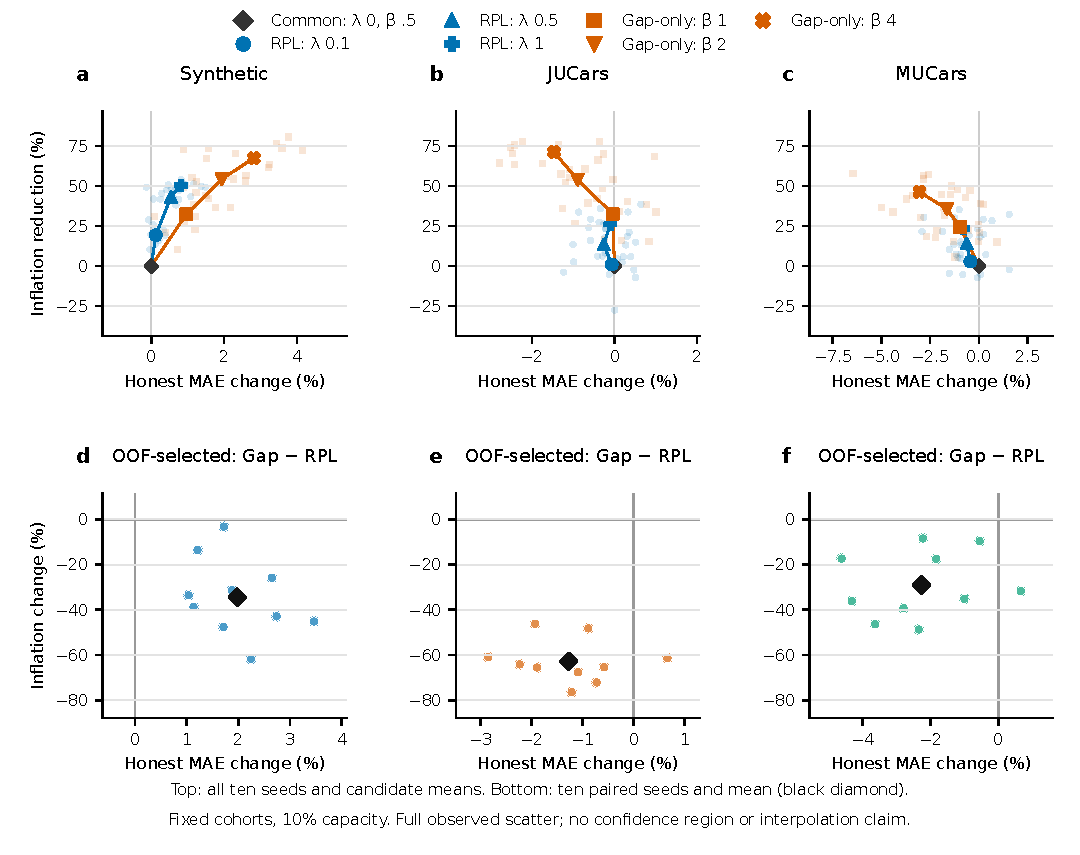
\includegraphics[width=\textwidth]{figures/review-v1/gap-tradeoffs.pdf}
\caption{Complete candidate and selected trade-offs at 10\% capacity.
(a--c) All seven unique candidates over ten fitting seeds. Pale points are
individual fits; colored symbols are means of same-seed percentage changes
relative to the common $(\lambda,\beta)=(0,.5)$ control. The common point
coincides at the origin; connecting lines only guide the candidate order.
Higher inflation reduction and lower honest-error change are favorable.
(d--f) Ten same-seed percentage changes from selected RPL to selected gap-only;
black diamonds are their means. Lower values on both axes are favorable.
These means of seed ratios differ from the ratios of source means in the
main text. Full observed scatter represents fitting variation, with no
confidence region or population extrapolation. Synthetic trades lower
inflation for higher error; the real-source means improve on both axes.}
\label{fig:stronger_gap_tradeoffs}
\end{figure}
\paragraph{Evidence and interpretation.}
Model, checkpoint, outcome and training-selection hashes bind the comparisons;
new-cell inflation and both MAE metrics are independently reaggregated from
saved outcomes. All 360 fit-stage records retain the two six-epoch updates
and declared gap/path settings. A separate implementation imports no runner
and independently checks the candidate sets, constraints and sixty choices
from saved OOF scalar scores; it does not regenerate OOF predictions.
This is a bounded computational check, not a new complete four-stage audit.
The complete grid, scores, selected cells and paired contrasts are released
under \path{notes/review-improvement-v1/gap/}. Scalar receipts are archived
separately, excluding weights, arrays and listing-level outcomes.

The comparison does not support practical superiority of RPL over a tuned
gap penalty on these cohorts. It also does not test stronger-gap combinations
with the five acquisition families: that separate 90-cell crossing holds
$\beta=.5$ and tests a different question. The graph loss remains a concrete
recovery-targeted formulation; its incremental benefit beyond stronger
gap regularization is unestablished under the present selection protocol.

\section{Numerical portability and retained failure}
An independently operated Mac completed the original six synthetic/seed-13
cells. Strict numerical reproduction failed under the original tolerances;
that verdict is retained. The ten-percent paired absolute improvement is
about .008024 locally and .008823 externally (53.97\% versus 57.54\%).
Direction agreement in one seed is supportive, but response quality differs:
$\lambda=1$ maximum regret changes from .0002041 to .0219727 at 10\% capacity.
The table distinguishes outcome direction from numerical equivalence.
\begin{table}[htbp]
\centering\small
\caption{Existing external-machine numerical comparison, synthetic seed 13. Each entry is local reference / external value. Strict numerical reproduction failed under the original tolerances.}
\label{tab:external-numerical}
\begin{tabular}{rrlll}
\toprule $\lambda$ & Capacity & Inflation (log) & Honest MAE & Attacked MAE\\\midrule
0 & 0\% & 0.0175119/0.0178126 & 3585.594/3582.048 & 3720.837/3714.437\\
0 & 10\% & 0.0148686/0.0153343 & 3585.594/3582.048 & 3688.439/3683.640\\
0 & 30\% & 0.0128125/0.0131494 & 3585.594/3582.048 & 3665.819/3661.133\\
1 & 0\% & 0.0121968/0.0119582 & 3615.223/3615.545 & 3676.134/3674.371\\
1 & 10\% & 0.0068443/0.0065113 & 3615.223/3615.545 & 3634.360/3621.562\\
1 & 30\% & 0.0041750/0.0041850 & 3615.223/3615.545 & 3616.811/3620.643\\
\midrule $\lambda$ & Capacity & Failed query (\%) & Maximum regret (log) & Nonconverged batches /10\\\midrule
0 & 0\% & 0.00/0.00 & 0.0000000/0.0000000 & 0/0\\
0 & 10\% & 2.70/2.50 & 0.0000000/0.0000000 & 0/0\\
0 & 30\% & 5.40/5.40 & 0.0000000/0.0000000 & 0/0\\
1 & 0\% & 0.00/0.00 & 0.0000000/0.0000000 & 0/0\\
1 & 10\% & 3.80/3.90 & 0.0002041/0.0219727 & 1/1\\
1 & 30\% & 7.60/7.40 & 0.0020809/0.0142298 & 1/2\\
\bottomrule\end{tabular}
\end{table}

Inputs and tree backbones matched; residual parameters differed. Each machine
was internally repeatable in the recorded repeats and thread comparisons.
The first recorded difference was an output-layer gradient; hidden forward
activations were not captured, so no underlying operator is causally isolated.
An isolated float64 candidate is not adopted or validated for scientific
performance. We neither relax tolerances nor retroactively substitute a new
scientific-equivalence criterion. No new external real-source comparison is
claimed. A stronger transportability claim requires a future locked protocol
and actual independent environment, including effect and regret checks.

The public \texttt{reproduction/macos-core-v2} and
\texttt{reproduction/windows-core-v1} directories contain minimal core training
procedures and data routes. The archived software excludes model weights and
listing-level outputs; it is not a self-contained binary model package.

\section{Version and evidence map}
The immutable software ZIP at
\href{https://doi.org/10.5281/zenodo.23447567}{10.5281/zenodo.23447567}
is version 1.0.0 from source \texttt{89ad56e}. It includes the earlier
90-cell crossing and external difference tables; it excludes manuscripts,
large weights, raw data and listing-level outcomes. Later paper revisions
and the present diagnostics are not retroactively inside that archive.
Current repository citation metadata follows the author order explicitly
confirmed by the authors: Tang, You (corresponding), Gu, Pang.

\begin{itemize}
\item Pre-review integrated paper: commit \texttt{45c2aef}; this is the earlier
28-page manuscript with the five-family crossing in its main text.
\item Matched gap runner and engineering replay: commit \texttt{5fb3437};
\path{experiments/run_review_gap_controls_v1.py} and its immutable manifest.
\item Mechanisms and cohort construction: commit \texttt{00eb579};
\path{notes/review-improvement-v1/}. Sixty models and 180 existing outcome
cells are newly diagnosed, not newly trained.
\item Equivalent no-feedback optimization: commit \texttt{7d870c2};
\path{experiments/run_review_gap_controls_v2.py}. The v1 checkpoints remain
bound and reusable; the engineering equivalence check precedes continuation.
\item Complete stronger-gap analysis and independent selection check:
commit \texttt{c7a577a}; all 90 new cells, 360 fit records and 210 candidates.
The complete trade-off figure and its rendered checks are in \texttt{2638dee}.
\item Current artifact hashes: \path{notes/review-improvement-v1/qa.json}.
They bind saved files; they do not establish scientific validity.
\end{itemize}
The main text and this supplement bound claims to the observed fixed
populations and declared response procedure. Fitting seeds do not sample
new training populations, and independent new-market effectiveness remains
unestablished.
\section{Full removals, default scans and seed heterogeneity}\label{app:extended}
The original component experiment toggles suppression scoring ($S$), feedback
($F$) and gap loss ($G$). All eight configurations retain backbone,
augmentation, error and anchoring terms, with equal role separation and epoch
budgets. Thus removal of two or all three components is evaluated against a
trained baseline (Figure~\ref{fig:completion_ablation}). These switches do
not constitute three independently established innovations.

Figure~\ref{fig:rpl_seeds} retains all ten fitting seeds and four nonzero
path/gap comparisons, each with its same-gap zero-path reference. Negative
seed effects at smaller weights remain. A separate original \emph{three-seed}
recovery-edge pilot found mean positive increments decreasing from .001790
to .000693 (synthetic), .001648 to .001048 (JUCars) and .000788 to .000450
(MUCars) at $\lambda=1,\beta=.5$. All remained positive: zero path loss was
not achieved, and the pilot is not relabeled as ten-seed evidence.

Core scans vary gap weight $0,.1,.25,.5,1,2$, tolerance
$0,.01,.02,.05,.1$ and feedback rounds $1,2,4$, at 10/30\% budgets.
Implementation scans vary anchoring, attack weight, learning rate, epochs,
head trees and width. Figures~\ref{fig:completion_parameters} and
\ref{fig:completion_stability} explicitly mark every scanned value and
engineering default; matching default observations are reused exactly, not
retrained or selected on evaluation outcomes. These three-seed scans do not
retune ten-seed RPL or prove an optimum. The separate availability stress
adds 0/10/30\% natural absence to fixed models (189 cells, 63 reused), with
seven policies and fresh response search but no new fitting; it is a controlled
perturbation rather than a new market or actual-seller validation.

\begin{figure}[p]\centering
\resizebox{\textwidth}{!}{%
\begingroup
\setlength{\unitlength}{1bp}
\begin{picture}(518.4000,244.8000)
\put(0,0){\AuditVector{q 0.5000 w 0.0000 0.0000 0.0000 RG 1.0000 1.0000 1.0000 rg [] 0 d 0.0000 0.0000 518.4000 244.8000 re f Q}}
\put(0,0){\AuditVector{q 0.5000 w 0.0000 0.0000 0.0000 RG 1.0000 1.0000 1.0000 rg [] 0 d 72.5760 48.9600 108.8640 154.2240 re f Q}}
\put(0,0){\AuditVector{q 0.8000 w 0.0000 0.0000 0.0000 RG 0.0000 0.0000 0.0000 rg [] 0 d 89.3835 48.9600 m 89.3835 45.4600 l B Q}}
\put(0,0){\AuditVector{q 0.8000 w 0.0000 0.0000 0.0000 RG 0.0000 0.0000 0.0000 rg [] 0 d 117.2589 48.9600 m 117.2589 45.4600 l B Q}}
\put(0,0){\AuditVector{q 0.8000 w 0.0000 0.0000 0.0000 RG 0.0000 0.0000 0.0000 rg [] 0 d 145.1343 48.9600 m 145.1343 45.4600 l B Q}}
\put(0,0){\AuditVector{q 0.8000 w 0.0000 0.0000 0.0000 RG 0.0000 0.0000 0.0000 rg [] 0 d 173.0097 48.9600 m 173.0097 45.4600 l B Q}}
\put(0,0){\AuditVector{q 0.4000 w 0.8666 0.8667 0.8666 RG [] 0 d 72.5760 193.6633 m 181.4400 193.6633 l S Q}}
\put(0,0){\AuditVector{q 0.8000 w 0.0000 0.0000 0.0000 RG 0.0000 0.0000 0.0000 rg [] 0 d 72.5760 193.6633 m 69.0760 193.6633 l B Q}}
\put(0,0){\AuditVector{q 0.4000 w 0.8666 0.8667 0.8666 RG [] 0 d 72.5760 174.3515 m 181.4400 174.3515 l S Q}}
\put(0,0){\AuditVector{q 0.8000 w 0.0000 0.0000 0.0000 RG 0.0000 0.0000 0.0000 rg [] 0 d 72.5760 174.3515 m 69.0760 174.3515 l B Q}}
\put(0,0){\AuditVector{q 0.4000 w 0.8666 0.8667 0.8666 RG [] 0 d 72.5760 155.0397 m 181.4400 155.0397 l S Q}}
\put(0,0){\AuditVector{q 0.8000 w 0.0000 0.0000 0.0000 RG 0.0000 0.0000 0.0000 rg [] 0 d 72.5760 155.0397 m 69.0760 155.0397 l B Q}}
\put(0,0){\AuditVector{q 0.4000 w 0.8666 0.8667 0.8666 RG [] 0 d 72.5760 135.7279 m 181.4400 135.7279 l S Q}}
\put(0,0){\AuditVector{q 0.8000 w 0.0000 0.0000 0.0000 RG 0.0000 0.0000 0.0000 rg [] 0 d 72.5760 135.7279 m 69.0760 135.7279 l B Q}}
\put(0,0){\AuditVector{q 0.4000 w 0.8666 0.8667 0.8666 RG [] 0 d 72.5760 116.4161 m 181.4400 116.4161 l S Q}}
\put(0,0){\AuditVector{q 0.8000 w 0.0000 0.0000 0.0000 RG 0.0000 0.0000 0.0000 rg [] 0 d 72.5760 116.4161 m 69.0760 116.4161 l B Q}}
\put(0,0){\AuditVector{q 0.4000 w 0.8666 0.8667 0.8666 RG [] 0 d 72.5760 97.1043 m 181.4400 97.1043 l S Q}}
\put(0,0){\AuditVector{q 0.8000 w 0.0000 0.0000 0.0000 RG 0.0000 0.0000 0.0000 rg [] 0 d 72.5760 97.1043 m 69.0760 97.1043 l B Q}}
\put(0,0){\AuditVector{q 0.4000 w 0.8666 0.8667 0.8666 RG [] 0 d 72.5760 77.7925 m 181.4400 77.7925 l S Q}}
\put(0,0){\AuditVector{q 0.8000 w 0.0000 0.0000 0.0000 RG 0.0000 0.0000 0.0000 rg [] 0 d 72.5760 77.7925 m 69.0760 77.7925 l B Q}}
\put(0,0){\AuditVector{q 0.4000 w 0.8666 0.8667 0.8666 RG [] 0 d 72.5760 58.4807 m 181.4400 58.4807 l S Q}}
\put(0,0){\AuditVector{q 0.8000 w 0.0000 0.0000 0.0000 RG 0.0000 0.0000 0.0000 rg [] 0 d 72.5760 58.4807 m 69.0760 58.4807 l B Q}}
\put(0,0){\AuditVector{q 0.7000 w 0.4666 0.4667 0.4666 RG [ 2.59 1.12 ] 0 d 117.2589 48.9600 m 117.2589 203.1840 l S Q}}
\put(0,0){\AuditVector{q 1.0000 w 0.4500 0.6959 0.8339 RG 0.4500 0.6959 0.8339 rg [] 0 d 139.3239 194.6738 m 139.7217 194.6738 140.1033 194.8319 140.3846 195.1132 c 140.6659 195.3944 140.8239 195.7760 140.8239 196.1738 c 140.8239 196.5716 140.6659 196.9532 140.3846 197.2345 c 140.1033 197.5158 139.7217 197.6738 139.3239 197.6738 c 138.9261 197.6738 138.5446 197.5158 138.2633 197.2345 c 137.9820 196.9532 137.8239 196.5716 137.8239 196.1738 c 137.8239 195.7760 137.9820 195.3944 138.2633 195.1132 c 138.5446 194.8319 138.9261 194.6738 139.3239 194.6738 c B Q}}
\put(0,0){\AuditVector{q 1.0000 w 0.4500 0.6959 0.8339 RG 0.4500 0.6959 0.8339 rg [] 0 d 124.7087 192.1633 m 125.1066 192.1633 125.4881 192.3213 125.7694 192.6026 c 126.0507 192.8839 126.2087 193.2655 126.2087 193.6633 c 126.2087 194.0611 126.0507 194.4426 125.7694 194.7239 c 125.4881 195.0052 125.1066 195.1633 124.7087 195.1633 c 124.3109 195.1633 123.9294 195.0052 123.6481 194.7239 c 123.3668 194.4426 123.2087 194.0611 123.2087 193.6633 c 123.2087 193.2655 123.3668 192.8839 123.6481 192.6026 c 123.9294 192.3213 124.3109 192.1633 124.7087 192.1633 c B Q}}
\put(0,0){\AuditVector{q 1.0000 w 0.4500 0.6959 0.8339 RG 0.4500 0.6959 0.8339 rg [] 0 d 130.2936 189.6527 m 130.6914 189.6527 131.0730 189.8108 131.3543 190.0921 c 131.6356 190.3734 131.7936 190.7549 131.7936 191.1527 c 131.7936 191.5506 131.6356 191.9321 131.3543 192.2134 c 131.0730 192.4947 130.6914 192.6527 130.2936 192.6527 c 129.8958 192.6527 129.5143 192.4947 129.2330 192.2134 c 128.9517 191.9321 128.7936 191.5506 128.7936 191.1527 c 128.7936 190.7549 128.9517 190.3734 129.2330 190.0921 c 129.5143 189.8108 129.8958 189.6527 130.2936 189.6527 c B Q}}
\put(0,0){\AuditVector{q 1.0000 w 0.0000 0.4471 0.6980 RG 0.0000 0.4471 0.6980 rg [] 0 d 131.4421 190.8349 m 134.2705 193.6633 l 131.4421 196.4917 l 128.6137 193.6633 l 131.4421 190.8349 l B Q}}
\put(0,0){\AuditVector{q 1.0000 w 0.4500 0.6959 0.8339 RG 0.4500 0.6959 0.8339 rg [] 0 d 97.1652 175.3620 m 97.5630 175.3620 97.9445 175.5201 98.2258 175.8014 c 98.5071 176.0826 98.6652 176.4642 98.6652 176.8620 c 98.6652 177.2598 98.5071 177.6414 98.2258 177.9227 c 97.9445 178.2040 97.5630 178.3620 97.1652 178.3620 c 96.7673 178.3620 96.3858 178.2040 96.1045 177.9227 c 95.8232 177.6414 95.6652 177.2598 95.6652 176.8620 c 95.6652 176.4642 95.8232 176.0826 96.1045 175.8014 c 96.3858 175.5201 96.7673 175.3620 97.1652 175.3620 c B Q}}
\put(0,0){\AuditVector{q 1.0000 w 0.4500 0.6959 0.8339 RG 0.4500 0.6959 0.8339 rg [] 0 d 77.5244 172.8515 m 77.9222 172.8515 78.3037 173.0095 78.5850 173.2908 c 78.8663 173.5721 79.0244 173.9537 79.0244 174.3515 c 79.0244 174.7493 78.8663 175.1309 78.5850 175.4121 c 78.3037 175.6934 77.9222 175.8515 77.5244 175.8515 c 77.1266 175.8515 76.7450 175.6934 76.4637 175.4121 c 76.1824 175.1309 76.0244 174.7493 76.0244 174.3515 c 76.0244 173.9537 76.1824 173.5721 76.4637 173.2908 c 76.7450 173.0095 77.1266 172.8515 77.5244 172.8515 c B Q}}
\put(0,0){\AuditVector{q 1.0000 w 0.4500 0.6959 0.8339 RG 0.4500 0.6959 0.8339 rg [] 0 d 87.9798 170.3409 m 88.3776 170.3409 88.7592 170.4990 89.0405 170.7803 c 89.3218 171.0616 89.4798 171.4431 89.4798 171.8409 c 89.4798 172.2387 89.3218 172.6203 89.0405 172.9016 c 88.7592 173.1829 88.3776 173.3409 87.9798 173.3409 c 87.5820 173.3409 87.2004 173.1829 86.9192 172.9016 c 86.6379 172.6203 86.4798 172.2387 86.4798 171.8409 c 86.4798 171.4431 86.6379 171.0616 86.9192 170.7803 c 87.2004 170.4990 87.5820 170.3409 87.9798 170.3409 c B Q}}
\put(0,0){\AuditVector{q 1.0000 w 0.0000 0.4471 0.6980 RG 0.0000 0.4471 0.6980 rg [] 0 d 87.5564 171.5231 m 90.3849 174.3515 l 87.5564 177.1799 l 84.7280 174.3515 l 87.5564 171.5231 l B Q}}
\put(0,0){\AuditVector{q 1.0000 w 0.4500 0.6959 0.8339 RG 0.4500 0.6959 0.8339 rg [] 0 d 176.4916 156.0502 m 176.8895 156.0502 177.2710 156.2083 177.5523 156.4896 c 177.8336 156.7709 177.9916 157.1524 177.9916 157.5502 c 177.9916 157.9480 177.8336 158.3296 177.5523 158.6109 c 177.2710 158.8922 176.8895 159.0502 176.4916 159.0502 c 176.0938 159.0502 175.7123 158.8922 175.4310 158.6109 c 175.1497 158.3296 174.9916 157.9480 174.9916 157.5502 c 174.9916 157.1524 175.1497 156.7709 175.4310 156.4896 c 175.7123 156.2083 176.0938 156.0502 176.4916 156.0502 c B Q}}
\put(0,0){\AuditVector{q 1.0000 w 0.4500 0.6959 0.8339 RG 0.4500 0.6959 0.8339 rg [] 0 d 163.2785 153.5397 m 163.6763 153.5397 164.0579 153.6977 164.3392 153.9790 c 164.6205 154.2603 164.7785 154.6419 164.7785 155.0397 c 164.7785 155.4375 164.6205 155.8191 164.3392 156.1004 c 164.0579 156.3816 163.6763 156.5397 163.2785 156.5397 c 162.8807 156.5397 162.4991 156.3816 162.2178 156.1004 c 161.9366 155.8191 161.7785 155.4375 161.7785 155.0397 c 161.7785 154.6419 161.9366 154.2603 162.2178 153.9790 c 162.4991 153.6977 162.8807 153.5397 163.2785 153.5397 c B Q}}
\put(0,0){\AuditVector{q 1.0000 w 0.4500 0.6959 0.8339 RG 0.4500 0.6959 0.8339 rg [] 0 d 162.1895 151.0292 m 162.5873 151.0292 162.9688 151.1872 163.2501 151.4685 c 163.5314 151.7498 163.6895 152.1314 163.6895 152.5292 c 163.6895 152.9270 163.5314 153.3085 163.2501 153.5898 c 162.9688 153.8711 162.5873 154.0292 162.1895 154.0292 c 161.7917 154.0292 161.4101 153.8711 161.1288 153.5898 c 160.8475 153.3085 160.6895 152.9270 160.6895 152.5292 c 160.6895 152.1314 160.8475 151.7498 161.1288 151.4685 c 161.4101 151.1872 161.7917 151.0292 162.1895 151.0292 c B Q}}
\put(0,0){\AuditVector{q 1.0000 w 0.0000 0.4471 0.6980 RG 0.0000 0.4471 0.6980 rg [] 0 d 167.3199 152.2113 m 170.1483 155.0397 l 167.3199 157.8681 l 164.4914 155.0397 l 167.3199 152.2113 l B Q}}
\put(0,0){\AuditVector{q 1.0000 w 0.4500 0.6959 0.8339 RG 0.4500 0.6959 0.8339 rg [] 0 d 113.1305 136.7384 m 113.5283 136.7384 113.9098 136.8965 114.1911 137.1778 c 114.4724 137.4591 114.6305 137.8406 114.6305 138.2384 c 114.6305 138.6362 114.4724 139.0178 114.1911 139.2991 c 113.9098 139.5804 113.5283 139.7384 113.1305 139.7384 c 112.7327 139.7384 112.3511 139.5804 112.0698 139.2991 c 111.7885 139.0178 111.6305 138.6362 111.6305 138.2384 c 111.6305 137.8406 111.7885 137.4591 112.0698 137.1778 c 112.3511 136.8965 112.7327 136.7384 113.1305 136.7384 c B Q}}
\put(0,0){\AuditVector{q 1.0000 w 0.4500 0.6959 0.8339 RG 0.4500 0.6959 0.8339 rg [] 0 d 105.0748 134.2279 m 105.4726 134.2279 105.8542 134.3859 106.1355 134.6672 c 106.4167 134.9485 106.5748 135.3301 106.5748 135.7279 c 106.5748 136.1257 106.4167 136.5073 106.1355 136.7886 c 105.8542 137.0698 105.4726 137.2279 105.0748 137.2279 c 104.6770 137.2279 104.2954 137.0698 104.0141 136.7886 c 103.7328 136.5073 103.5748 136.1257 103.5748 135.7279 c 103.5748 135.3301 103.7328 134.9485 104.0141 134.6672 c 104.2954 134.3859 104.6770 134.2279 105.0748 134.2279 c B Q}}
\put(0,0){\AuditVector{q 1.0000 w 0.4500 0.6959 0.8339 RG 0.4500 0.6959 0.8339 rg [] 0 d 121.2659 131.7174 m 121.6637 131.7174 122.0453 131.8754 122.3266 132.1567 c 122.6079 132.4380 122.7659 132.8196 122.7659 133.2174 c 122.7659 133.6152 122.6079 133.9967 122.3266 134.2780 c 122.0453 134.5593 121.6637 134.7174 121.2659 134.7174 c 120.8681 134.7174 120.4865 134.5593 120.2052 134.2780 c 119.9240 133.9967 119.7659 133.6152 119.7659 133.2174 c 119.7659 132.8196 119.9240 132.4380 120.2052 132.1567 c 120.4865 131.8754 120.8681 131.7174 121.2659 131.7174 c B Q}}
\put(0,0){\AuditVector{q 1.0000 w 0.0000 0.4471 0.6980 RG 0.0000 0.4471 0.6980 rg [] 0 d 113.1571 132.8995 m 115.9855 135.7279 l 113.1571 138.5563 l 110.3286 135.7279 l 113.1571 132.8995 l B Q}}
\put(0,0){\AuditVector{q 1.0000 w 0.4500 0.6959 0.8339 RG 0.4500 0.6959 0.8339 rg [] 0 d 152.3839 117.4266 m 152.7817 117.4266 153.1633 117.5847 153.4445 117.8660 c 153.7258 118.1473 153.8839 118.5288 153.8839 118.9266 c 153.8839 119.3244 153.7258 119.7060 153.4445 119.9873 c 153.1633 120.2686 152.7817 120.4266 152.3839 120.4266 c 151.9861 120.4266 151.6045 120.2686 151.3232 119.9873 c 151.0419 119.7060 150.8839 119.3244 150.8839 118.9266 c 150.8839 118.5288 151.0419 118.1473 151.3232 117.8660 c 151.6045 117.5847 151.9861 117.4266 152.3839 117.4266 c B Q}}
\put(0,0){\AuditVector{q 1.0000 w 0.4500 0.6959 0.8339 RG 0.4500 0.6959 0.8339 rg [] 0 d 144.2007 114.9161 m 144.5985 114.9161 144.9801 115.0742 145.2613 115.3555 c 145.5426 115.6367 145.7007 116.0183 145.7007 116.4161 c 145.7007 116.8139 145.5426 117.1955 145.2613 117.4768 c 144.9801 117.7581 144.5985 117.9161 144.2007 117.9161 c 143.8029 117.9161 143.4213 117.7581 143.1400 117.4768 c 142.8587 117.1955 142.7007 116.8139 142.7007 116.4161 c 142.7007 116.0183 142.8587 115.6367 143.1400 115.3555 c 143.4213 115.0742 143.8029 114.9161 144.2007 114.9161 c B Q}}
\put(0,0){\AuditVector{q 1.0000 w 0.4500 0.6959 0.8339 RG 0.4500 0.6959 0.8339 rg [] 0 d 147.7239 112.4056 m 148.1217 112.4056 148.5033 112.5636 148.7846 112.8449 c 149.0659 113.1262 149.2239 113.5078 149.2239 113.9056 c 149.2239 114.3034 149.0659 114.6850 148.7846 114.9662 c 148.5033 115.2475 148.1217 115.4056 147.7239 115.4056 c 147.3261 115.4056 146.9446 115.2475 146.6633 114.9662 c 146.3820 114.6850 146.2239 114.3034 146.2239 113.9056 c 146.2239 113.5078 146.3820 113.1262 146.6633 112.8449 c 146.9446 112.5636 147.3261 112.4056 147.7239 112.4056 c B Q}}
\put(0,0){\AuditVector{q 1.0000 w 0.0000 0.4471 0.6980 RG 0.0000 0.4471 0.6980 rg [] 0 d 148.1028 113.5877 m 150.9313 116.4161 l 148.1028 119.2445 l 145.2744 116.4161 l 148.1028 113.5877 l B Q}}
\put(0,0){\AuditVector{q 1.0000 w 0.4500 0.6959 0.8339 RG 0.4500 0.6959 0.8339 rg [] 0 d 106.2364 98.1148 m 106.6342 98.1148 107.0158 98.2729 107.2971 98.5542 c 107.5784 98.8355 107.7364 99.2170 107.7364 99.6148 c 107.7364 100.0126 107.5784 100.3942 107.2971 100.6755 c 107.0158 100.9568 106.6342 101.1148 106.2364 101.1148 c 105.8386 101.1148 105.4571 100.9568 105.1758 100.6755 c 104.8945 100.3942 104.7364 100.0126 104.7364 99.6148 c 104.7364 99.2170 104.8945 98.8355 105.1758 98.5542 c 105.4571 98.2729 105.8386 98.1148 106.2364 98.1148 c B Q}}
\put(0,0){\AuditVector{q 1.0000 w 0.4500 0.6959 0.8339 RG 0.4500 0.6959 0.8339 rg [] 0 d 85.3620 95.6043 m 85.7598 95.6043 86.1414 95.7624 86.4227 96.0437 c 86.7040 96.3249 86.8620 96.7065 86.8620 97.1043 c 86.8620 97.5021 86.7040 97.8837 86.4227 98.1650 c 86.1414 98.4463 85.7598 98.6043 85.3620 98.6043 c 84.9642 98.6043 84.5827 98.4463 84.3014 98.1650 c 84.0201 97.8837 83.8620 97.5021 83.8620 97.1043 c 83.8620 96.7065 84.0201 96.3249 84.3014 96.0437 c 84.5827 95.7624 84.9642 95.6043 85.3620 95.6043 c B Q}}
\put(0,0){\AuditVector{q 1.0000 w 0.4500 0.6959 0.8339 RG 0.4500 0.6959 0.8339 rg [] 0 d 95.5663 93.0938 m 95.9641 93.0938 96.3457 93.2518 96.6270 93.5331 c 96.9083 93.8144 97.0663 94.1960 97.0663 94.5938 c 97.0663 94.9916 96.9083 95.3732 96.6270 95.6544 c 96.3457 95.9357 95.9641 96.0938 95.5663 96.0938 c 95.1685 96.0938 94.7870 95.9357 94.5057 95.6544 c 94.2244 95.3732 94.0663 94.9916 94.0663 94.5938 c 94.0663 94.1960 94.2244 93.8144 94.5057 93.5331 c 94.7870 93.2518 95.1685 93.0938 95.5663 93.0938 c B Q}}
\put(0,0){\AuditVector{q 1.0000 w 0.0000 0.4471 0.6980 RG 0.0000 0.4471 0.6980 rg [] 0 d 95.7216 94.2759 m 98.5500 97.1043 l 95.7216 99.9327 l 92.8932 97.1043 l 95.7216 94.2759 l B Q}}
\put(0,0){\AuditVector{q 1.0000 w 0.4500 0.6959 0.8339 RG 0.4500 0.6959 0.8339 rg [] 0 d 169.5462 78.8031 m 169.9440 78.8031 170.3256 78.9611 170.6068 79.2424 c 170.8881 79.5237 171.0462 79.9052 171.0462 80.3031 c 171.0462 80.7009 170.8881 81.0824 170.6068 81.3637 c 170.3256 81.6450 169.9440 81.8031 169.5462 81.8031 c 169.1484 81.8031 168.7668 81.6450 168.4855 81.3637 c 168.2042 81.0824 168.0462 80.7009 168.0462 80.3031 c 168.0462 79.9052 168.2042 79.5237 168.4855 79.2424 c 168.7668 78.9611 169.1484 78.8031 169.5462 78.8031 c B Q}}
\put(0,0){\AuditVector{q 1.0000 w 0.4500 0.6959 0.8339 RG 0.4500 0.6959 0.8339 rg [] 0 d 169.4803 76.2925 m 169.8781 76.2925 170.2597 76.4506 170.5409 76.7319 c 170.8222 77.0132 170.9803 77.3947 170.9803 77.7925 c 170.9803 78.1903 170.8222 78.5719 170.5409 78.8532 c 170.2597 79.1345 169.8781 79.2925 169.4803 79.2925 c 169.0825 79.2925 168.7009 79.1345 168.4196 78.8532 c 168.1383 78.5719 167.9803 78.1903 167.9803 77.7925 c 167.9803 77.3947 168.1383 77.0132 168.4196 76.7319 c 168.7009 76.4506 169.0825 76.2925 169.4803 76.2925 c B Q}}
\put(0,0){\AuditVector{q 1.0000 w 0.4500 0.6959 0.8339 RG 0.4500 0.6959 0.8339 rg [] 0 d 166.4622 73.7820 m 166.8600 73.7820 167.2415 73.9400 167.5228 74.2213 c 167.8041 74.5026 167.9622 74.8842 167.9622 75.2820 c 167.9622 75.6798 167.8041 76.0614 167.5228 76.3427 c 167.2415 76.6239 166.8600 76.7820 166.4622 76.7820 c 166.0644 76.7820 165.6828 76.6239 165.4015 76.3427 c 165.1202 76.0614 164.9622 75.6798 164.9622 75.2820 c 164.9622 74.8842 165.1202 74.5026 165.4015 74.2213 c 165.6828 73.9400 166.0644 73.7820 166.4622 73.7820 c B Q}}
\put(0,0){\AuditVector{q 1.0000 w 0.0000 0.4471 0.6980 RG 0.0000 0.4471 0.6980 rg [] 0 d 168.4962 74.9641 m 171.3246 77.7925 l 168.4962 80.6209 l 165.6678 77.7925 l 168.4962 74.9641 l B Q}}
\put(0,0){\AuditVector{q 1.0000 w 0.4500 0.6959 0.8339 RG 0.4500 0.6959 0.8339 rg [] 0 d 117.2589 59.4913 m 117.6567 59.4913 118.0383 59.6493 118.3196 59.9306 c 118.6009 60.2119 118.7589 60.5934 118.7589 60.9913 c 118.7589 61.3891 118.6009 61.7706 118.3196 62.0519 c 118.0383 62.3332 117.6567 62.4913 117.2589 62.4913 c 116.8611 62.4913 116.4795 62.3332 116.1982 62.0519 c 115.9170 61.7706 115.7589 61.3891 115.7589 60.9913 c 115.7589 60.5934 115.9170 60.2119 116.1982 59.9306 c 116.4795 59.6493 116.8611 59.4913 117.2589 59.4913 c B Q}}
\put(0,0){\AuditVector{q 1.0000 w 0.4500 0.6959 0.8339 RG 0.4500 0.6959 0.8339 rg [] 0 d 117.2589 56.9807 m 117.6567 56.9807 118.0383 57.1388 118.3196 57.4201 c 118.6009 57.7014 118.7589 58.0829 118.7589 58.4807 c 118.7589 58.8785 118.6009 59.2601 118.3196 59.5414 c 118.0383 59.8227 117.6567 59.9807 117.2589 59.9807 c 116.8611 59.9807 116.4795 59.8227 116.1982 59.5414 c 115.9170 59.2601 115.7589 58.8785 115.7589 58.4807 c 115.7589 58.0829 115.9170 57.7014 116.1982 57.4201 c 116.4795 57.1388 116.8611 56.9807 117.2589 56.9807 c B Q}}
\put(0,0){\AuditVector{q 1.0000 w 0.4500 0.6959 0.8339 RG 0.4500 0.6959 0.8339 rg [] 0 d 117.2589 54.4702 m 117.6567 54.4702 118.0383 54.6283 118.3196 54.9095 c 118.6009 55.1908 118.7589 55.5724 118.7589 55.9702 c 118.7589 56.3680 118.6009 56.7496 118.3196 57.0309 c 118.0383 57.3121 117.6567 57.4702 117.2589 57.4702 c 116.8611 57.4702 116.4795 57.3121 116.1982 57.0309 c 115.9170 56.7496 115.7589 56.3680 115.7589 55.9702 c 115.7589 55.5724 115.9170 55.1908 116.1982 54.9095 c 116.4795 54.6283 116.8611 54.4702 117.2589 54.4702 c B Q}}
\put(0,0){\AuditVector{q 1.0000 w 0.0000 0.4471 0.6980 RG 0.0000 0.4471 0.6980 rg [] 0 d 117.2589 55.6523 m 120.0873 58.4807 l 117.2589 61.3091 l 114.4305 58.4807 l 117.2589 55.6523 l B Q}}
\put(0,0){\AuditVector{q 0.7000 w 0.0000 0.0000 0.0000 RG [] 0 d 72.5760 48.9600 m 72.5760 203.1840 l S Q}}
\put(0,0){\AuditVector{q 0.7000 w 0.0000 0.0000 0.0000 RG [] 0 d 72.5760 48.9600 m 181.4400 48.9600 l S Q}}
\put(0,0){\AuditVector{q 0.5000 w 0.0000 0.0000 0.0000 RG 1.0000 1.0000 1.0000 rg [] 0 d 235.8720 48.9600 108.8640 154.2240 re f Q}}
\put(0,0){\AuditVector{q 0.8000 w 0.0000 0.0000 0.0000 RG 0.0000 0.0000 0.0000 rg [] 0 d 249.9884 48.9600 m 249.9884 45.4600 l B Q}}
\put(0,0){\AuditVector{q 0.8000 w 0.0000 0.0000 0.0000 RG 0.0000 0.0000 0.0000 rg [] 0 d 282.8859 48.9600 m 282.8859 45.4600 l B Q}}
\put(0,0){\AuditVector{q 0.8000 w 0.0000 0.0000 0.0000 RG 0.0000 0.0000 0.0000 rg [] 0 d 315.7835 48.9600 m 315.7835 45.4600 l B Q}}
\put(0,0){\AuditVector{q 0.4000 w 0.8666 0.8667 0.8666 RG [] 0 d 235.8720 193.6633 m 344.7360 193.6633 l S Q}}
\put(0,0){\AuditVector{q 0.8000 w 0.0000 0.0000 0.0000 RG 0.0000 0.0000 0.0000 rg [] 0 d 235.8720 193.6633 m 232.3720 193.6633 l B Q}}
\put(0,0){\AuditVector{q 0.4000 w 0.8666 0.8667 0.8666 RG [] 0 d 235.8720 174.3515 m 344.7360 174.3515 l S Q}}
\put(0,0){\AuditVector{q 0.8000 w 0.0000 0.0000 0.0000 RG 0.0000 0.0000 0.0000 rg [] 0 d 235.8720 174.3515 m 232.3720 174.3515 l B Q}}
\put(0,0){\AuditVector{q 0.4000 w 0.8666 0.8667 0.8666 RG [] 0 d 235.8720 155.0397 m 344.7360 155.0397 l S Q}}
\put(0,0){\AuditVector{q 0.8000 w 0.0000 0.0000 0.0000 RG 0.0000 0.0000 0.0000 rg [] 0 d 235.8720 155.0397 m 232.3720 155.0397 l B Q}}
\put(0,0){\AuditVector{q 0.4000 w 0.8666 0.8667 0.8666 RG [] 0 d 235.8720 135.7279 m 344.7360 135.7279 l S Q}}
\put(0,0){\AuditVector{q 0.8000 w 0.0000 0.0000 0.0000 RG 0.0000 0.0000 0.0000 rg [] 0 d 235.8720 135.7279 m 232.3720 135.7279 l B Q}}
\put(0,0){\AuditVector{q 0.4000 w 0.8666 0.8667 0.8666 RG [] 0 d 235.8720 116.4161 m 344.7360 116.4161 l S Q}}
\put(0,0){\AuditVector{q 0.8000 w 0.0000 0.0000 0.0000 RG 0.0000 0.0000 0.0000 rg [] 0 d 235.8720 116.4161 m 232.3720 116.4161 l B Q}}
\put(0,0){\AuditVector{q 0.4000 w 0.8666 0.8667 0.8666 RG [] 0 d 235.8720 97.1043 m 344.7360 97.1043 l S Q}}
\put(0,0){\AuditVector{q 0.8000 w 0.0000 0.0000 0.0000 RG 0.0000 0.0000 0.0000 rg [] 0 d 235.8720 97.1043 m 232.3720 97.1043 l B Q}}
\put(0,0){\AuditVector{q 0.4000 w 0.8666 0.8667 0.8666 RG [] 0 d 235.8720 77.7925 m 344.7360 77.7925 l S Q}}
\put(0,0){\AuditVector{q 0.8000 w 0.0000 0.0000 0.0000 RG 0.0000 0.0000 0.0000 rg [] 0 d 235.8720 77.7925 m 232.3720 77.7925 l B Q}}
\put(0,0){\AuditVector{q 0.4000 w 0.8666 0.8667 0.8666 RG [] 0 d 235.8720 58.4807 m 344.7360 58.4807 l S Q}}
\put(0,0){\AuditVector{q 0.8000 w 0.0000 0.0000 0.0000 RG 0.0000 0.0000 0.0000 rg [] 0 d 235.8720 58.4807 m 232.3720 58.4807 l B Q}}
\put(0,0){\AuditVector{q 0.7000 w 0.4666 0.4667 0.4666 RG [ 2.59 1.12 ] 0 d 249.9884 48.9600 m 249.9884 203.1840 l S Q}}
\put(0,0){\AuditVector{q 1.0000 w 0.9094 0.6527 0.4500 RG 0.9094 0.6527 0.4500 rg [] 0 d 290.9476 194.6738 m 291.3454 194.6738 291.7270 194.8319 292.0083 195.1132 c 292.2896 195.3944 292.4476 195.7760 292.4476 196.1738 c 292.4476 196.5716 292.2896 196.9532 292.0083 197.2345 c 291.7270 197.5158 291.3454 197.6738 290.9476 197.6738 c 290.5498 197.6738 290.1683 197.5158 289.8870 197.2345 c 289.6057 196.9532 289.4476 196.5716 289.4476 196.1738 c 289.4476 195.7760 289.6057 195.3944 289.8870 195.1132 c 290.1683 194.8319 290.5498 194.6738 290.9476 194.6738 c B Q}}
\put(0,0){\AuditVector{q 1.0000 w 0.9094 0.6527 0.4500 RG 0.9094 0.6527 0.4500 rg [] 0 d 318.8972 192.1633 m 319.2950 192.1633 319.6766 192.3213 319.9579 192.6026 c 320.2392 192.8839 320.3972 193.2655 320.3972 193.6633 c 320.3972 194.0611 320.2392 194.4426 319.9579 194.7239 c 319.6766 195.0052 319.2950 195.1633 318.8972 195.1633 c 318.4994 195.1633 318.1179 195.0052 317.8365 194.7239 c 317.5553 194.4426 317.3972 194.0611 317.3972 193.6633 c 317.3972 193.2655 317.5553 192.8839 317.8365 192.6026 c 318.1179 192.3213 318.4994 192.1633 318.8972 192.1633 c B Q}}
\put(0,0){\AuditVector{q 1.0000 w 0.9094 0.6527 0.4500 RG 0.9094 0.6527 0.4500 rg [] 0 d 284.4518 189.6527 m 284.8496 189.6527 285.2312 189.8108 285.5125 190.0921 c 285.7938 190.3734 285.9518 190.7549 285.9518 191.1527 c 285.9518 191.5506 285.7938 191.9321 285.5125 192.2134 c 285.2312 192.4947 284.8496 192.6527 284.4518 192.6527 c 284.0540 192.6527 283.6725 192.4947 283.3911 192.2134 c 283.1099 191.9321 282.9518 191.5506 282.9518 191.1527 c 282.9518 190.7549 283.1099 190.3734 283.3911 190.0921 c 283.6725 189.8108 284.0540 189.6527 284.4518 189.6527 c B Q}}
\put(0,0){\AuditVector{q 1.0000 w 0.8353 0.3686 0.0000 RG 0.8353 0.3686 0.0000 rg [] 0 d 298.0989 190.8349 m 300.9273 193.6633 l 298.0989 196.4917 l 295.2704 193.6633 l 298.0989 190.8349 l B Q}}
\put(0,0){\AuditVector{q 1.0000 w 0.9094 0.6527 0.4500 RG 0.9094 0.6527 0.4500 rg [] 0 d 245.8701 175.3620 m 246.2679 175.3620 246.6495 175.5201 246.9308 175.8014 c 247.2121 176.0826 247.3701 176.4642 247.3701 176.8620 c 247.3701 177.2598 247.2121 177.6414 246.9308 177.9227 c 246.6495 178.2040 246.2679 178.3620 245.8701 178.3620 c 245.4723 178.3620 245.0907 178.2040 244.8094 177.9227 c 244.5282 177.6414 244.3701 177.2598 244.3701 176.8620 c 244.3701 176.4642 244.5282 176.0826 244.8094 175.8014 c 245.0907 175.5201 245.4723 175.3620 245.8701 175.3620 c B Q}}
\put(0,0){\AuditVector{q 1.0000 w 0.9094 0.6527 0.4500 RG 0.9094 0.6527 0.4500 rg [] 0 d 240.8204 172.8515 m 241.2182 172.8515 241.5997 173.0095 241.8810 173.2908 c 242.1623 173.5721 242.3204 173.9537 242.3204 174.3515 c 242.3204 174.7493 242.1623 175.1309 241.8810 175.4121 c 241.5997 175.6934 241.2182 175.8515 240.8204 175.8515 c 240.4225 175.8515 240.0410 175.6934 239.7597 175.4121 c 239.4784 175.1309 239.3204 174.7493 239.3204 174.3515 c 239.3204 173.9537 239.4784 173.5721 239.7597 173.2908 c 240.0410 173.0095 240.4225 172.8515 240.8204 172.8515 c B Q}}
\put(0,0){\AuditVector{q 1.0000 w 0.9094 0.6527 0.4500 RG 0.9094 0.6527 0.4500 rg [] 0 d 243.0705 170.3409 m 243.4683 170.3409 243.8499 170.4990 244.1312 170.7803 c 244.4125 171.0616 244.5705 171.4431 244.5705 171.8409 c 244.5705 172.2387 244.4125 172.6203 244.1312 172.9016 c 243.8499 173.1829 243.4683 173.3409 243.0705 173.3409 c 242.6727 173.3409 242.2911 173.1829 242.0099 172.9016 c 241.7286 172.6203 241.5705 172.2387 241.5705 171.8409 c 241.5705 171.4431 241.7286 171.0616 242.0099 170.7803 c 242.2911 170.4990 242.6727 170.3409 243.0705 170.3409 c B Q}}
\put(0,0){\AuditVector{q 1.0000 w 0.8353 0.3686 0.0000 RG 0.8353 0.3686 0.0000 rg [] 0 d 243.2537 171.5231 m 246.0821 174.3515 l 243.2537 177.1799 l 240.4252 174.3515 l 243.2537 171.5231 l B Q}}
\put(0,0){\AuditVector{q 1.0000 w 0.9094 0.6527 0.4500 RG 0.9094 0.6527 0.4500 rg [] 0 d 289.9291 156.0502 m 290.3269 156.0502 290.7085 156.2083 290.9898 156.4896 c 291.2711 156.7709 291.4291 157.1524 291.4291 157.5502 c 291.4291 157.9480 291.2711 158.3296 290.9898 158.6109 c 290.7085 158.8922 290.3269 159.0502 289.9291 159.0502 c 289.5313 159.0502 289.1497 158.8922 288.8684 158.6109 c 288.5872 158.3296 288.4291 157.9480 288.4291 157.5502 c 288.4291 157.1524 288.5872 156.7709 288.8684 156.4896 c 289.1497 156.2083 289.5313 156.0502 289.9291 156.0502 c B Q}}
\put(0,0){\AuditVector{q 1.0000 w 0.9094 0.6527 0.4500 RG 0.9094 0.6527 0.4500 rg [] 0 d 339.7876 153.5397 m 340.1854 153.5397 340.5670 153.6977 340.8483 153.9790 c 341.1296 154.2603 341.2876 154.6419 341.2876 155.0397 c 341.2876 155.4375 341.1296 155.8191 340.8483 156.1004 c 340.5670 156.3816 340.1854 156.5397 339.7876 156.5397 c 339.3898 156.5397 339.0083 156.3816 338.7270 156.1004 c 338.4457 155.8191 338.2876 155.4375 338.2876 155.0397 c 338.2876 154.6419 338.4457 154.2603 338.7270 153.9790 c 339.0083 153.6977 339.3898 153.5397 339.7876 153.5397 c B Q}}
\put(0,0){\AuditVector{q 1.0000 w 0.9094 0.6527 0.4500 RG 0.9094 0.6527 0.4500 rg [] 0 d 313.3095 151.0292 m 313.7073 151.0292 314.0888 151.1872 314.3701 151.4685 c 314.6514 151.7498 314.8095 152.1314 314.8095 152.5292 c 314.8095 152.9270 314.6514 153.3085 314.3701 153.5898 c 314.0888 153.8711 313.7073 154.0292 313.3095 154.0292 c 312.9117 154.0292 312.5301 153.8711 312.2488 153.5898 c 311.9675 153.3085 311.8095 152.9270 311.8095 152.5292 c 311.8095 152.1314 311.9675 151.7498 312.2488 151.4685 c 312.5301 151.1872 312.9117 151.0292 313.3095 151.0292 c B Q}}
\put(0,0){\AuditVector{q 1.0000 w 0.8353 0.3686 0.0000 RG 0.8353 0.3686 0.0000 rg [] 0 d 314.3421 152.2113 m 317.1705 155.0397 l 314.3421 157.8681 l 311.5136 155.0397 l 314.3421 152.2113 l B Q}}
\put(0,0){\AuditVector{q 1.0000 w 0.9094 0.6527 0.4500 RG 0.9094 0.6527 0.4500 rg [] 0 d 253.3593 136.7384 m 253.7571 136.7384 254.1387 136.8965 254.4200 137.1778 c 254.7013 137.4591 254.8593 137.8406 254.8593 138.2384 c 254.8593 138.6362 254.7013 139.0178 254.4200 139.2991 c 254.1387 139.5804 253.7571 139.7384 253.3593 139.7384 c 252.9615 139.7384 252.5800 139.5804 252.2987 139.2991 c 252.0174 139.0178 251.8593 138.6362 251.8593 138.2384 c 251.8593 137.8406 252.0174 137.4591 252.2987 137.1778 c 252.5800 136.8965 252.9615 136.7384 253.3593 136.7384 c B Q}}
\put(0,0){\AuditVector{q 1.0000 w 0.9094 0.6527 0.4500 RG 0.9094 0.6527 0.4500 rg [] 0 d 263.6612 134.2279 m 264.0590 134.2279 264.4406 134.3859 264.7219 134.6672 c 265.0032 134.9485 265.1612 135.3301 265.1612 135.7279 c 265.1612 136.1257 265.0032 136.5073 264.7219 136.7886 c 264.4406 137.0698 264.0590 137.2279 263.6612 137.2279 c 263.2634 137.2279 262.8819 137.0698 262.6006 136.7886 c 262.3193 136.5073 262.1612 136.1257 262.1612 135.7279 c 262.1612 135.3301 262.3193 134.9485 262.6006 134.6672 c 262.8819 134.3859 263.2634 134.2279 263.6612 134.2279 c B Q}}
\put(0,0){\AuditVector{q 1.0000 w 0.9094 0.6527 0.4500 RG 0.9094 0.6527 0.4500 rg [] 0 d 258.7586 131.7174 m 259.1564 131.7174 259.5380 131.8754 259.8193 132.1567 c 260.1006 132.4380 260.2586 132.8196 260.2586 133.2174 c 260.2586 133.6152 260.1006 133.9967 259.8193 134.2780 c 259.5380 134.5593 259.1564 134.7174 258.7586 134.7174 c 258.3608 134.7174 257.9793 134.5593 257.6980 134.2780 c 257.4167 133.9967 257.2586 133.6152 257.2586 133.2174 c 257.2586 132.8196 257.4167 132.4380 257.6980 132.1567 c 257.9793 131.8754 258.3608 131.7174 258.7586 131.7174 c B Q}}
\put(0,0){\AuditVector{q 1.0000 w 0.8353 0.3686 0.0000 RG 0.8353 0.3686 0.0000 rg [] 0 d 258.5931 132.8995 m 261.4215 135.7279 l 258.5931 138.5563 l 255.7646 135.7279 l 258.5931 132.8995 l B Q}}
\put(0,0){\AuditVector{q 1.0000 w 0.9094 0.6527 0.4500 RG 0.9094 0.6527 0.4500 rg [] 0 d 291.8032 117.4266 m 292.2010 117.4266 292.5825 117.5847 292.8638 117.8660 c 293.1451 118.1473 293.3032 118.5288 293.3032 118.9266 c 293.3032 119.3244 293.1451 119.7060 292.8638 119.9873 c 292.5825 120.2686 292.2010 120.4266 291.8032 120.4266 c 291.4054 120.4266 291.0238 120.2686 290.7425 119.9873 c 290.4612 119.7060 290.3032 119.3244 290.3032 118.9266 c 290.3032 118.5288 290.4612 118.1473 290.7425 117.8660 c 291.0238 117.5847 291.4054 117.4266 291.8032 117.4266 c B Q}}
\put(0,0){\AuditVector{q 1.0000 w 0.9094 0.6527 0.4500 RG 0.9094 0.6527 0.4500 rg [] 0 d 314.0353 114.9161 m 314.4331 114.9161 314.8147 115.0742 315.0960 115.3555 c 315.3773 115.6367 315.5353 116.0183 315.5353 116.4161 c 315.5353 116.8139 315.3773 117.1955 315.0960 117.4768 c 314.8147 117.7581 314.4331 117.9161 314.0353 117.9161 c 313.6375 117.9161 313.2560 117.7581 312.9746 117.4768 c 312.6934 117.1955 312.5353 116.8139 312.5353 116.4161 c 312.5353 116.0183 312.6934 115.6367 312.9746 115.3555 c 313.2560 115.0742 313.6375 114.9161 314.0353 114.9161 c B Q}}
\put(0,0){\AuditVector{q 1.0000 w 0.9094 0.6527 0.4500 RG 0.9094 0.6527 0.4500 rg [] 0 d 285.7489 112.4056 m 286.1467 112.4056 286.5283 112.5636 286.8096 112.8449 c 287.0909 113.1262 287.2489 113.5078 287.2489 113.9056 c 287.2489 114.3034 287.0909 114.6850 286.8096 114.9662 c 286.5283 115.2475 286.1467 115.4056 285.7489 115.4056 c 285.3511 115.4056 284.9696 115.2475 284.6883 114.9662 c 284.4070 114.6850 284.2489 114.3034 284.2489 113.9056 c 284.2489 113.5078 284.4070 113.1262 284.6883 112.8449 c 284.9696 112.5636 285.3511 112.4056 285.7489 112.4056 c B Q}}
\put(0,0){\AuditVector{q 1.0000 w 0.8353 0.3686 0.0000 RG 0.8353 0.3686 0.0000 rg [] 0 d 297.1958 113.5877 m 300.0242 116.4161 l 297.1958 119.2445 l 294.3674 116.4161 l 297.1958 113.5877 l B Q}}
\put(0,0){\AuditVector{q 1.0000 w 0.9094 0.6527 0.4500 RG 0.9094 0.6527 0.4500 rg [] 0 d 244.6665 98.1148 m 245.0643 98.1148 245.4459 98.2729 245.7272 98.5542 c 246.0085 98.8355 246.1665 99.2170 246.1665 99.6148 c 246.1665 100.0126 246.0085 100.3942 245.7272 100.6755 c 245.4459 100.9568 245.0643 101.1148 244.6665 101.1148 c 244.2687 101.1148 243.8872 100.9568 243.6059 100.6755 c 243.3246 100.3942 243.1665 100.0126 243.1665 99.6148 c 243.1665 99.2170 243.3246 98.8355 243.6059 98.5542 c 243.8872 98.2729 244.2687 98.1148 244.6665 98.1148 c B Q}}
\put(0,0){\AuditVector{q 1.0000 w 0.9094 0.6527 0.4500 RG 0.9094 0.6527 0.4500 rg [] 0 d 244.1581 95.6043 m 244.5559 95.6043 244.9375 95.7624 245.2187 96.0437 c 245.5000 96.3249 245.6581 96.7065 245.6581 97.1043 c 245.6581 97.5021 245.5000 97.8837 245.2187 98.1650 c 244.9375 98.4463 244.5559 98.6043 244.1581 98.6043 c 243.7603 98.6043 243.3787 98.4463 243.0974 98.1650 c 242.8161 97.8837 242.6581 97.5021 242.6581 97.1043 c 242.6581 96.7065 242.8161 96.3249 243.0974 96.0437 c 243.3787 95.7624 243.7603 95.6043 244.1581 95.6043 c B Q}}
\put(0,0){\AuditVector{q 1.0000 w 0.9094 0.6527 0.4500 RG 0.9094 0.6527 0.4500 rg [] 0 d 244.4910 93.0938 m 244.8888 93.0938 245.2704 93.2518 245.5517 93.5331 c 245.8329 93.8144 245.9910 94.1960 245.9910 94.5938 c 245.9910 94.9916 245.8329 95.3732 245.5517 95.6544 c 245.2704 95.9357 244.8888 96.0938 244.4910 96.0938 c 244.0932 96.0938 243.7116 95.9357 243.4303 95.6544 c 243.1490 95.3732 242.9910 94.9916 242.9910 94.5938 c 242.9910 94.1960 243.1490 93.8144 243.4303 93.5331 c 243.7116 93.2518 244.0932 93.0938 244.4910 93.0938 c B Q}}
\put(0,0){\AuditVector{q 1.0000 w 0.8353 0.3686 0.0000 RG 0.8353 0.3686 0.0000 rg [] 0 d 244.4385 94.2759 m 247.2670 97.1043 l 244.4385 99.9327 l 241.6101 97.1043 l 244.4385 94.2759 l B Q}}
\put(0,0){\AuditVector{q 1.0000 w 0.9094 0.6527 0.4500 RG 0.9094 0.6527 0.4500 rg [] 0 d 285.2982 78.8031 m 285.6960 78.8031 286.0776 78.9611 286.3589 79.2424 c 286.6402 79.5237 286.7982 79.9052 286.7982 80.3031 c 286.7982 80.7009 286.6402 81.0824 286.3589 81.3637 c 286.0776 81.6450 285.6960 81.8031 285.2982 81.8031 c 284.9004 81.8031 284.5189 81.6450 284.2375 81.3637 c 283.9563 81.0824 283.7982 80.7009 283.7982 80.3031 c 283.7982 79.9052 283.9563 79.5237 284.2375 79.2424 c 284.5189 78.9611 284.9004 78.8031 285.2982 78.8031 c B Q}}
\put(0,0){\AuditVector{q 1.0000 w 0.9094 0.6527 0.4500 RG 0.9094 0.6527 0.4500 rg [] 0 d 331.4411 76.2925 m 331.8389 76.2925 332.2204 76.4506 332.5017 76.7319 c 332.7830 77.0132 332.9411 77.3947 332.9411 77.7925 c 332.9411 78.1903 332.7830 78.5719 332.5017 78.8532 c 332.2204 79.1345 331.8389 79.2925 331.4411 79.2925 c 331.0433 79.2925 330.6617 79.1345 330.3804 78.8532 c 330.0991 78.5719 329.9411 78.1903 329.9411 77.7925 c 329.9411 77.3947 330.0991 77.0132 330.3804 76.7319 c 330.6617 76.4506 331.0433 76.2925 331.4411 76.2925 c B Q}}
\put(0,0){\AuditVector{q 1.0000 w 0.9094 0.6527 0.4500 RG 0.9094 0.6527 0.4500 rg [] 0 d 305.5803 73.7820 m 305.9781 73.7820 306.3596 73.9400 306.6409 74.2213 c 306.9222 74.5026 307.0803 74.8842 307.0803 75.2820 c 307.0803 75.6798 306.9222 76.0614 306.6409 76.3427 c 306.3596 76.6239 305.9781 76.7820 305.5803 76.7820 c 305.1825 76.7820 304.8009 76.6239 304.5196 76.3427 c 304.2383 76.0614 304.0803 75.6798 304.0803 75.2820 c 304.0803 74.8842 304.2383 74.5026 304.5196 74.2213 c 304.8009 73.9400 305.1825 73.7820 305.5803 73.7820 c B Q}}
\put(0,0){\AuditVector{q 1.0000 w 0.8353 0.3686 0.0000 RG 0.8353 0.3686 0.0000 rg [] 0 d 307.4399 74.9641 m 310.2683 77.7925 l 307.4399 80.6209 l 304.6115 77.7925 l 307.4399 74.9641 l B Q}}
\put(0,0){\AuditVector{q 1.0000 w 0.9094 0.6527 0.4500 RG 0.9094 0.6527 0.4500 rg [] 0 d 249.9884 59.4913 m 250.3862 59.4913 250.7678 59.6493 251.0490 59.9306 c 251.3303 60.2119 251.4884 60.5934 251.4884 60.9913 c 251.4884 61.3891 251.3303 61.7706 251.0490 62.0519 c 250.7678 62.3332 250.3862 62.4913 249.9884 62.4913 c 249.5906 62.4913 249.2090 62.3332 248.9277 62.0519 c 248.6464 61.7706 248.4884 61.3891 248.4884 60.9913 c 248.4884 60.5934 248.6464 60.2119 248.9277 59.9306 c 249.2090 59.6493 249.5906 59.4913 249.9884 59.4913 c B Q}}
\put(0,0){\AuditVector{q 1.0000 w 0.9094 0.6527 0.4500 RG 0.9094 0.6527 0.4500 rg [] 0 d 249.9884 56.9807 m 250.3862 56.9807 250.7678 57.1388 251.0490 57.4201 c 251.3303 57.7014 251.4884 58.0829 251.4884 58.4807 c 251.4884 58.8785 251.3303 59.2601 251.0490 59.5414 c 250.7678 59.8227 250.3862 59.9807 249.9884 59.9807 c 249.5906 59.9807 249.2090 59.8227 248.9277 59.5414 c 248.6464 59.2601 248.4884 58.8785 248.4884 58.4807 c 248.4884 58.0829 248.6464 57.7014 248.9277 57.4201 c 249.2090 57.1388 249.5906 56.9807 249.9884 56.9807 c B Q}}
\put(0,0){\AuditVector{q 1.0000 w 0.9094 0.6527 0.4500 RG 0.9094 0.6527 0.4500 rg [] 0 d 249.9884 54.4702 m 250.3862 54.4702 250.7678 54.6283 251.0490 54.9095 c 251.3303 55.1908 251.4884 55.5724 251.4884 55.9702 c 251.4884 56.3680 251.3303 56.7496 251.0490 57.0309 c 250.7678 57.3121 250.3862 57.4702 249.9884 57.4702 c 249.5906 57.4702 249.2090 57.3121 248.9277 57.0309 c 248.6464 56.7496 248.4884 56.3680 248.4884 55.9702 c 248.4884 55.5724 248.6464 55.1908 248.9277 54.9095 c 249.2090 54.6283 249.5906 54.4702 249.9884 54.4702 c B Q}}
\put(0,0){\AuditVector{q 1.0000 w 0.8353 0.3686 0.0000 RG 0.8353 0.3686 0.0000 rg [] 0 d 249.9884 55.6523 m 252.8168 58.4807 l 249.9884 61.3091 l 247.1600 58.4807 l 249.9884 55.6523 l B Q}}
\put(0,0){\AuditVector{q 0.7000 w 0.0000 0.0000 0.0000 RG [] 0 d 235.8720 48.9600 m 235.8720 203.1840 l S Q}}
\put(0,0){\AuditVector{q 0.7000 w 0.0000 0.0000 0.0000 RG [] 0 d 235.8720 48.9600 m 344.7360 48.9600 l S Q}}
\put(0,0){\AuditVector{q 0.5000 w 0.0000 0.0000 0.0000 RG 1.0000 1.0000 1.0000 rg [] 0 d 399.1680 48.9600 108.8640 154.2240 re f Q}}
\put(0,0){\AuditVector{q 0.8000 w 0.0000 0.0000 0.0000 RG 0.0000 0.0000 0.0000 rg [] 0 d 406.3851 48.9600 m 406.3851 45.4600 l B Q}}
\put(0,0){\AuditVector{q 0.8000 w 0.0000 0.0000 0.0000 RG 0.0000 0.0000 0.0000 rg [] 0 d 457.7968 48.9600 m 457.7968 45.4600 l B Q}}
\put(0,0){\AuditVector{q 0.4000 w 0.8666 0.8667 0.8666 RG [] 0 d 399.1680 193.6633 m 508.0320 193.6633 l S Q}}
\put(0,0){\AuditVector{q 0.8000 w 0.0000 0.0000 0.0000 RG 0.0000 0.0000 0.0000 rg [] 0 d 399.1680 193.6633 m 395.6680 193.6633 l B Q}}
\put(0,0){\AuditVector{q 0.4000 w 0.8666 0.8667 0.8666 RG [] 0 d 399.1680 174.3515 m 508.0320 174.3515 l S Q}}
\put(0,0){\AuditVector{q 0.8000 w 0.0000 0.0000 0.0000 RG 0.0000 0.0000 0.0000 rg [] 0 d 399.1680 174.3515 m 395.6680 174.3515 l B Q}}
\put(0,0){\AuditVector{q 0.4000 w 0.8666 0.8667 0.8666 RG [] 0 d 399.1680 155.0397 m 508.0320 155.0397 l S Q}}
\put(0,0){\AuditVector{q 0.8000 w 0.0000 0.0000 0.0000 RG 0.0000 0.0000 0.0000 rg [] 0 d 399.1680 155.0397 m 395.6680 155.0397 l B Q}}
\put(0,0){\AuditVector{q 0.4000 w 0.8666 0.8667 0.8666 RG [] 0 d 399.1680 135.7279 m 508.0320 135.7279 l S Q}}
\put(0,0){\AuditVector{q 0.8000 w 0.0000 0.0000 0.0000 RG 0.0000 0.0000 0.0000 rg [] 0 d 399.1680 135.7279 m 395.6680 135.7279 l B Q}}
\put(0,0){\AuditVector{q 0.4000 w 0.8666 0.8667 0.8666 RG [] 0 d 399.1680 116.4161 m 508.0320 116.4161 l S Q}}
\put(0,0){\AuditVector{q 0.8000 w 0.0000 0.0000 0.0000 RG 0.0000 0.0000 0.0000 rg [] 0 d 399.1680 116.4161 m 395.6680 116.4161 l B Q}}
\put(0,0){\AuditVector{q 0.4000 w 0.8666 0.8667 0.8666 RG [] 0 d 399.1680 97.1043 m 508.0320 97.1043 l S Q}}
\put(0,0){\AuditVector{q 0.8000 w 0.0000 0.0000 0.0000 RG 0.0000 0.0000 0.0000 rg [] 0 d 399.1680 97.1043 m 395.6680 97.1043 l B Q}}
\put(0,0){\AuditVector{q 0.4000 w 0.8666 0.8667 0.8666 RG [] 0 d 399.1680 77.7925 m 508.0320 77.7925 l S Q}}
\put(0,0){\AuditVector{q 0.8000 w 0.0000 0.0000 0.0000 RG 0.0000 0.0000 0.0000 rg [] 0 d 399.1680 77.7925 m 395.6680 77.7925 l B Q}}
\put(0,0){\AuditVector{q 0.4000 w 0.8666 0.8667 0.8666 RG [] 0 d 399.1680 58.4807 m 508.0320 58.4807 l S Q}}
\put(0,0){\AuditVector{q 0.8000 w 0.0000 0.0000 0.0000 RG 0.0000 0.0000 0.0000 rg [] 0 d 399.1680 58.4807 m 395.6680 58.4807 l B Q}}
\put(0,0){\AuditVector{q 0.7000 w 0.4666 0.4667 0.4666 RG [ 2.59 1.12 ] 0 d 406.3851 48.9600 m 406.3851 203.1840 l S Q}}
\put(0,0){\AuditVector{q 1.0000 w 0.4500 0.7908 0.6980 RG 0.4500 0.7908 0.6980 rg [] 0 d 465.8211 194.6738 m 466.2189 194.6738 466.6004 194.8319 466.8817 195.1132 c 467.1630 195.3944 467.3211 195.7760 467.3211 196.1738 c 467.3211 196.5716 467.1630 196.9532 466.8817 197.2345 c 466.6004 197.5158 466.2189 197.6738 465.8211 197.6738 c 465.4233 197.6738 465.0417 197.5158 464.7604 197.2345 c 464.4791 196.9532 464.3211 196.5716 464.3211 196.1738 c 464.3211 195.7760 464.4791 195.3944 464.7604 195.1132 c 465.0417 194.8319 465.4233 194.6738 465.8211 194.6738 c B Q}}
\put(0,0){\AuditVector{q 1.0000 w 0.4500 0.7908 0.6980 RG 0.4500 0.7908 0.6980 rg [] 0 d 467.3894 192.1633 m 467.7872 192.1633 468.1688 192.3213 468.4501 192.6026 c 468.7314 192.8839 468.8894 193.2655 468.8894 193.6633 c 468.8894 194.0611 468.7314 194.4426 468.4501 194.7239 c 468.1688 195.0052 467.7872 195.1633 467.3894 195.1633 c 466.9916 195.1633 466.6101 195.0052 466.3288 194.7239 c 466.0475 194.4426 465.8894 194.0611 465.8894 193.6633 c 465.8894 193.2655 466.0475 192.8839 466.3288 192.6026 c 466.6101 192.3213 466.9916 192.1633 467.3894 192.1633 c B Q}}
\put(0,0){\AuditVector{q 1.0000 w 0.4500 0.7908 0.6980 RG 0.4500 0.7908 0.6980 rg [] 0 d 491.3043 189.6527 m 491.7021 189.6527 492.0837 189.8108 492.3650 190.0921 c 492.6463 190.3734 492.8043 190.7549 492.8043 191.1527 c 492.8043 191.5506 492.6463 191.9321 492.3650 192.2134 c 492.0837 192.4947 491.7021 192.6527 491.3043 192.6527 c 490.9065 192.6527 490.5250 192.4947 490.2437 192.2134 c 489.9624 191.9321 489.8043 191.5506 489.8043 191.1527 c 489.8043 190.7549 489.9624 190.3734 490.2437 190.0921 c 490.5250 189.8108 490.9065 189.6527 491.3043 189.6527 c B Q}}
\put(0,0){\AuditVector{q 1.0000 w 0.0000 0.6196 0.4510 RG 0.0000 0.6196 0.4510 rg [] 0 d 474.8383 190.8349 m 477.6667 193.6633 l 474.8383 196.4917 l 472.0099 193.6633 l 474.8383 190.8349 l B Q}}
\put(0,0){\AuditVector{q 1.0000 w 0.4500 0.7908 0.6980 RG 0.4500 0.7908 0.6980 rg [] 0 d 405.2618 175.3620 m 405.6596 175.3620 406.0412 175.5201 406.3225 175.8014 c 406.6038 176.0826 406.7618 176.4642 406.7618 176.8620 c 406.7618 177.2598 406.6038 177.6414 406.3225 177.9227 c 406.0412 178.2040 405.6596 178.3620 405.2618 178.3620 c 404.8640 178.3620 404.4825 178.2040 404.2012 177.9227 c 403.9199 177.6414 403.7618 177.2598 403.7618 176.8620 c 403.7618 176.4642 403.9199 176.0826 404.2012 175.8014 c 404.4825 175.5201 404.8640 175.3620 405.2618 175.3620 c B Q}}
\put(0,0){\AuditVector{q 1.0000 w 0.4500 0.7908 0.6980 RG 0.4500 0.7908 0.6980 rg [] 0 d 405.5286 172.8515 m 405.9264 172.8515 406.3079 173.0095 406.5892 173.2908 c 406.8705 173.5721 407.0286 173.9537 407.0286 174.3515 c 407.0286 174.7493 406.8705 175.1309 406.5892 175.4121 c 406.3079 175.6934 405.9264 175.8515 405.5286 175.8515 c 405.1308 175.8515 404.7492 175.6934 404.4679 175.4121 c 404.1866 175.1309 404.0286 174.7493 404.0286 174.3515 c 404.0286 173.9537 404.1866 173.5721 404.4679 173.2908 c 404.7492 173.0095 405.1308 172.8515 405.5286 172.8515 c B Q}}
\put(0,0){\AuditVector{q 1.0000 w 0.4500 0.7908 0.6980 RG 0.4500 0.7908 0.6980 rg [] 0 d 404.1164 170.3409 m 404.5142 170.3409 404.8958 170.4990 405.1771 170.7803 c 405.4583 171.0616 405.6164 171.4431 405.6164 171.8409 c 405.6164 172.2387 405.4583 172.6203 405.1771 172.9016 c 404.8958 173.1829 404.5142 173.3409 404.1164 173.3409 c 403.7186 173.3409 403.3370 173.1829 403.0557 172.9016 c 402.7744 172.6203 402.6164 172.2387 402.6164 171.8409 c 402.6164 171.4431 402.7744 171.0616 403.0557 170.7803 c 403.3370 170.4990 403.7186 170.3409 404.1164 170.3409 c B Q}}
\put(0,0){\AuditVector{q 1.0000 w 0.0000 0.6196 0.4510 RG 0.0000 0.6196 0.4510 rg [] 0 d 404.9689 171.5231 m 407.7973 174.3515 l 404.9689 177.1799 l 402.1405 174.3515 l 404.9689 171.5231 l B Q}}
\put(0,0){\AuditVector{q 1.0000 w 0.4500 0.7908 0.6980 RG 0.4500 0.7908 0.6980 rg [] 0 d 472.0601 156.0502 m 472.4579 156.0502 472.8394 156.2083 473.1207 156.4896 c 473.4020 156.7709 473.5601 157.1524 473.5601 157.5502 c 473.5601 157.9480 473.4020 158.3296 473.1207 158.6109 c 472.8394 158.8922 472.4579 159.0502 472.0601 159.0502 c 471.6623 159.0502 471.2807 158.8922 470.9994 158.6109 c 470.7181 158.3296 470.5601 157.9480 470.5601 157.5502 c 470.5601 157.1524 470.7181 156.7709 470.9994 156.4896 c 471.2807 156.2083 471.6623 156.0502 472.0601 156.0502 c B Q}}
\put(0,0){\AuditVector{q 1.0000 w 0.4500 0.7908 0.6980 RG 0.4500 0.7908 0.6980 rg [] 0 d 479.5544 153.5397 m 479.9522 153.5397 480.3338 153.6977 480.6151 153.9790 c 480.8964 154.2603 481.0544 154.6419 481.0544 155.0397 c 481.0544 155.4375 480.8964 155.8191 480.6151 156.1004 c 480.3338 156.3816 479.9522 156.5397 479.5544 156.5397 c 479.1566 156.5397 478.7751 156.3816 478.4938 156.1004 c 478.2125 155.8191 478.0544 155.4375 478.0544 155.0397 c 478.0544 154.6419 478.2125 154.2603 478.4938 153.9790 c 478.7751 153.6977 479.1566 153.5397 479.5544 153.5397 c B Q}}
\put(0,0){\AuditVector{q 1.0000 w 0.4500 0.7908 0.6980 RG 0.4500 0.7908 0.6980 rg [] 0 d 498.1656 151.0292 m 498.5634 151.0292 498.9450 151.1872 499.2263 151.4685 c 499.5076 151.7498 499.6656 152.1314 499.6656 152.5292 c 499.6656 152.9270 499.5076 153.3085 499.2263 153.5898 c 498.9450 153.8711 498.5634 154.0292 498.1656 154.0292 c 497.7678 154.0292 497.3863 153.8711 497.1049 153.5898 c 496.8237 153.3085 496.6656 152.9270 496.6656 152.5292 c 496.6656 152.1314 496.8237 151.7498 497.1049 151.4685 c 497.3863 151.1872 497.7678 151.0292 498.1656 151.0292 c B Q}}
\put(0,0){\AuditVector{q 1.0000 w 0.0000 0.6196 0.4510 RG 0.0000 0.6196 0.4510 rg [] 0 d 483.2600 152.2113 m 486.0885 155.0397 l 483.2600 157.8681 l 480.4316 155.0397 l 483.2600 152.2113 l B Q}}
\put(0,0){\AuditVector{q 1.0000 w 0.4500 0.7908 0.6980 RG 0.4500 0.7908 0.6980 rg [] 0 d 408.5024 136.7384 m 408.9002 136.7384 409.2818 136.8965 409.5631 137.1778 c 409.8444 137.4591 410.0024 137.8406 410.0024 138.2384 c 410.0024 138.6362 409.8444 139.0178 409.5631 139.2991 c 409.2818 139.5804 408.9002 139.7384 408.5024 139.7384 c 408.1046 139.7384 407.7231 139.5804 407.4418 139.2991 c 407.1605 139.0178 407.0024 138.6362 407.0024 138.2384 c 407.0024 137.8406 407.1605 137.4591 407.4418 137.1778 c 407.7231 136.8965 408.1046 136.7384 408.5024 136.7384 c B Q}}
\put(0,0){\AuditVector{q 1.0000 w 0.4500 0.7908 0.6980 RG 0.4500 0.7908 0.6980 rg [] 0 d 411.3154 134.2279 m 411.7132 134.2279 412.0948 134.3859 412.3761 134.6672 c 412.6574 134.9485 412.8154 135.3301 412.8154 135.7279 c 412.8154 136.1257 412.6574 136.5073 412.3761 136.7886 c 412.0948 137.0698 411.7132 137.2279 411.3154 137.2279 c 410.9176 137.2279 410.5361 137.0698 410.2548 136.7886 c 409.9735 136.5073 409.8154 136.1257 409.8154 135.7279 c 409.8154 135.3301 409.9735 134.9485 410.2548 134.6672 c 410.5361 134.3859 410.9176 134.2279 411.3154 134.2279 c B Q}}
\put(0,0){\AuditVector{q 1.0000 w 0.4500 0.7908 0.6980 RG 0.4500 0.7908 0.6980 rg [] 0 d 409.1422 131.7174 m 409.5400 131.7174 409.9215 131.8754 410.2029 132.1567 c 410.4841 132.4380 410.6422 132.8196 410.6422 133.2174 c 410.6422 133.6152 410.4841 133.9967 410.2029 134.2780 c 409.9215 134.5593 409.5400 134.7174 409.1422 134.7174 c 408.7444 134.7174 408.3628 134.5593 408.0815 134.2780 c 407.8002 133.9967 407.6422 133.6152 407.6422 133.2174 c 407.6422 132.8196 407.8002 132.4380 408.0815 132.1567 c 408.3628 131.8754 408.7444 131.7174 409.1422 131.7174 c B Q}}
\put(0,0){\AuditVector{q 1.0000 w 0.0000 0.6196 0.4510 RG 0.0000 0.6196 0.4510 rg [] 0 d 409.6534 132.8995 m 412.4818 135.7279 l 409.6534 138.5563 l 406.8249 135.7279 l 409.6534 132.8995 l B Q}}
\put(0,0){\AuditVector{q 1.0000 w 0.4500 0.7908 0.6980 RG 0.4500 0.7908 0.6980 rg [] 0 d 466.1357 117.4266 m 466.5335 117.4266 466.9151 117.5847 467.1964 117.8660 c 467.4777 118.1473 467.6357 118.5288 467.6357 118.9266 c 467.6357 119.3244 467.4777 119.7060 467.1964 119.9873 c 466.9151 120.2686 466.5335 120.4266 466.1357 120.4266 c 465.7379 120.4266 465.3564 120.2686 465.0750 119.9873 c 464.7938 119.7060 464.6357 119.3244 464.6357 118.9266 c 464.6357 118.5288 464.7938 118.1473 465.0750 117.8660 c 465.3564 117.5847 465.7379 117.4266 466.1357 117.4266 c B Q}}
\put(0,0){\AuditVector{q 1.0000 w 0.4500 0.7908 0.6980 RG 0.4500 0.7908 0.6980 rg [] 0 d 467.2897 114.9161 m 467.6875 114.9161 468.0691 115.0742 468.3504 115.3555 c 468.6317 115.6367 468.7897 116.0183 468.7897 116.4161 c 468.7897 116.8139 468.6317 117.1955 468.3504 117.4768 c 468.0691 117.7581 467.6875 117.9161 467.2897 117.9161 c 466.8919 117.9161 466.5103 117.7581 466.2290 117.4768 c 465.9478 117.1955 465.7897 116.8139 465.7897 116.4161 c 465.7897 116.0183 465.9478 115.6367 466.2290 115.3555 c 466.5103 115.0742 466.8919 114.9161 467.2897 114.9161 c B Q}}
\put(0,0){\AuditVector{q 1.0000 w 0.4500 0.7908 0.6980 RG 0.4500 0.7908 0.6980 rg [] 0 d 489.7971 112.4056 m 490.1949 112.4056 490.5765 112.5636 490.8578 112.8449 c 491.1391 113.1262 491.2971 113.5078 491.2971 113.9056 c 491.2971 114.3034 491.1391 114.6850 490.8578 114.9662 c 490.5765 115.2475 490.1949 115.4056 489.7971 115.4056 c 489.3993 115.4056 489.0178 115.2475 488.7365 114.9662 c 488.4552 114.6850 488.2971 114.3034 488.2971 113.9056 c 488.2971 113.5078 488.4552 113.1262 488.7365 112.8449 c 489.0178 112.5636 489.3993 112.4056 489.7971 112.4056 c B Q}}
\put(0,0){\AuditVector{q 1.0000 w 0.0000 0.6196 0.4510 RG 0.0000 0.6196 0.4510 rg [] 0 d 474.4075 113.5877 m 477.2359 116.4161 l 474.4075 119.2445 l 471.5791 116.4161 l 474.4075 113.5877 l B Q}}
\put(0,0){\AuditVector{q 1.0000 w 0.4500 0.7908 0.6980 RG 0.4500 0.7908 0.6980 rg [] 0 d 404.9702 98.1148 m 405.3680 98.1148 405.7496 98.2729 406.0309 98.5542 c 406.3122 98.8355 406.4702 99.2170 406.4702 99.6148 c 406.4702 100.0126 406.3122 100.3942 406.0309 100.6755 c 405.7496 100.9568 405.3680 101.1148 404.9702 101.1148 c 404.5724 101.1148 404.1909 100.9568 403.9096 100.6755 c 403.6283 100.3942 403.4702 100.0126 403.4702 99.6148 c 403.4702 99.2170 403.6283 98.8355 403.9096 98.5542 c 404.1909 98.2729 404.5724 98.1148 404.9702 98.1148 c B Q}}
\put(0,0){\AuditVector{q 1.0000 w 0.4500 0.7908 0.6980 RG 0.4500 0.7908 0.6980 rg [] 0 d 405.6667 95.6043 m 406.0645 95.6043 406.4460 95.7624 406.7274 96.0437 c 407.0086 96.3249 407.1667 96.7065 407.1667 97.1043 c 407.1667 97.5021 407.0086 97.8837 406.7274 98.1650 c 406.4460 98.4463 406.0645 98.6043 405.6667 98.6043 c 405.2689 98.6043 404.8873 98.4463 404.6060 98.1650 c 404.3247 97.8837 404.1667 97.5021 404.1667 97.1043 c 404.1667 96.7065 404.3247 96.3249 404.6060 96.0437 c 404.8873 95.7624 405.2689 95.6043 405.6667 95.6043 c B Q}}
\put(0,0){\AuditVector{q 1.0000 w 0.4500 0.7908 0.6980 RG 0.4500 0.7908 0.6980 rg [] 0 d 404.9204 93.0938 m 405.3182 93.0938 405.6998 93.2518 405.9811 93.5331 c 406.2624 93.8144 406.4204 94.1960 406.4204 94.5938 c 406.4204 94.9916 406.2624 95.3732 405.9811 95.6544 c 405.6998 95.9357 405.3182 96.0938 404.9204 96.0938 c 404.5226 96.0938 404.1411 95.9357 403.8598 95.6544 c 403.5785 95.3732 403.4204 94.9916 403.4204 94.5938 c 403.4204 94.1960 403.5785 93.8144 403.8598 93.5331 c 404.1411 93.2518 404.5226 93.0938 404.9204 93.0938 c B Q}}
\put(0,0){\AuditVector{q 1.0000 w 0.0000 0.6196 0.4510 RG 0.0000 0.6196 0.4510 rg [] 0 d 405.1858 94.2759 m 408.0142 97.1043 l 405.1858 99.9327 l 402.3574 97.1043 l 405.1858 94.2759 l B Q}}
\put(0,0){\AuditVector{q 1.0000 w 0.4500 0.7908 0.6980 RG 0.4500 0.7908 0.6980 rg [] 0 d 475.8285 78.8031 m 476.2263 78.8031 476.6079 78.9611 476.8892 79.2424 c 477.1705 79.5237 477.3285 79.9052 477.3285 80.3031 c 477.3285 80.7009 477.1705 81.0824 476.8892 81.3637 c 476.6079 81.6450 476.2263 81.8031 475.8285 81.8031 c 475.4307 81.8031 475.0492 81.6450 474.7679 81.3637 c 474.4866 81.0824 474.3285 80.7009 474.3285 80.3031 c 474.3285 79.9052 474.4866 79.5237 474.7679 79.2424 c 475.0492 78.9611 475.4307 78.8031 475.8285 78.8031 c B Q}}
\put(0,0){\AuditVector{q 1.0000 w 0.4500 0.7908 0.6980 RG 0.4500 0.7908 0.6980 rg [] 0 d 481.7293 76.2925 m 482.1271 76.2925 482.5087 76.4506 482.7900 76.7319 c 483.0713 77.0132 483.2293 77.3947 483.2293 77.7925 c 483.2293 78.1903 483.0713 78.5719 482.7900 78.8532 c 482.5087 79.1345 482.1271 79.2925 481.7293 79.2925 c 481.3315 79.2925 480.9500 79.1345 480.6686 78.8532 c 480.3874 78.5719 480.2293 78.1903 480.2293 77.7925 c 480.2293 77.3947 480.3874 77.0132 480.6686 76.7319 c 480.9500 76.4506 481.3315 76.2925 481.7293 76.2925 c B Q}}
\put(0,0){\AuditVector{q 1.0000 w 0.4500 0.7908 0.6980 RG 0.4500 0.7908 0.6980 rg [] 0 d 503.0836 73.7820 m 503.4814 73.7820 503.8630 73.9400 504.1443 74.2213 c 504.4256 74.5026 504.5836 74.8842 504.5836 75.2820 c 504.5836 75.6798 504.4256 76.0614 504.1443 76.3427 c 503.8630 76.6239 503.4814 76.7820 503.0836 76.7820 c 502.6859 76.7820 502.3043 76.6239 502.0230 76.3427 c 501.7417 76.0614 501.5836 75.6798 501.5836 75.2820 c 501.5836 74.8842 501.7417 74.5026 502.0230 74.2213 c 502.3043 73.9400 502.6859 73.7820 503.0836 73.7820 c B Q}}
\put(0,0){\AuditVector{q 1.0000 w 0.0000 0.6196 0.4510 RG 0.0000 0.6196 0.4510 rg [] 0 d 486.8805 74.9641 m 489.7089 77.7925 l 486.8805 80.6209 l 484.0521 77.7925 l 486.8805 74.9641 l B Q}}
\put(0,0){\AuditVector{q 1.0000 w 0.4500 0.7908 0.6980 RG 0.4500 0.7908 0.6980 rg [] 0 d 406.3851 59.4913 m 406.7829 59.4913 407.1644 59.6493 407.4457 59.9306 c 407.7270 60.2119 407.8851 60.5934 407.8851 60.9913 c 407.8851 61.3891 407.7270 61.7706 407.4457 62.0519 c 407.1644 62.3332 406.7829 62.4913 406.3851 62.4913 c 405.9873 62.4913 405.6057 62.3332 405.3244 62.0519 c 405.0431 61.7706 404.8851 61.3891 404.8851 60.9913 c 404.8851 60.5934 405.0431 60.2119 405.3244 59.9306 c 405.6057 59.6493 405.9873 59.4913 406.3851 59.4913 c B Q}}
\put(0,0){\AuditVector{q 1.0000 w 0.4500 0.7908 0.6980 RG 0.4500 0.7908 0.6980 rg [] 0 d 406.3851 56.9807 m 406.7829 56.9807 407.1644 57.1388 407.4457 57.4201 c 407.7270 57.7014 407.8851 58.0829 407.8851 58.4807 c 407.8851 58.8785 407.7270 59.2601 407.4457 59.5414 c 407.1644 59.8227 406.7829 59.9807 406.3851 59.9807 c 405.9873 59.9807 405.6057 59.8227 405.3244 59.5414 c 405.0431 59.2601 404.8851 58.8785 404.8851 58.4807 c 404.8851 58.0829 405.0431 57.7014 405.3244 57.4201 c 405.6057 57.1388 405.9873 56.9807 406.3851 56.9807 c B Q}}
\put(0,0){\AuditVector{q 1.0000 w 0.4500 0.7908 0.6980 RG 0.4500 0.7908 0.6980 rg [] 0 d 406.3851 54.4702 m 406.7829 54.4702 407.1644 54.6283 407.4457 54.9095 c 407.7270 55.1908 407.8851 55.5724 407.8851 55.9702 c 407.8851 56.3680 407.7270 56.7496 407.4457 57.0309 c 407.1644 57.3121 406.7829 57.4702 406.3851 57.4702 c 405.9873 57.4702 405.6057 57.3121 405.3244 57.0309 c 405.0431 56.7496 404.8851 56.3680 404.8851 55.9702 c 404.8851 55.5724 405.0431 55.1908 405.3244 54.9095 c 405.6057 54.6283 405.9873 54.4702 406.3851 54.4702 c B Q}}
\put(0,0){\AuditVector{q 1.0000 w 0.0000 0.6196 0.4510 RG 0.0000 0.6196 0.4510 rg [] 0 d 406.3851 55.6523 m 409.2135 58.4807 l 406.3851 61.3091 l 403.5566 58.4807 l 406.3851 55.6523 l B Q}}
\put(0,0){\AuditVector{q 0.7000 w 0.0000 0.0000 0.0000 RG [] 0 d 399.1680 48.9600 m 399.1680 203.1840 l S Q}}
\put(0,0){\AuditVector{q 0.7000 w 0.0000 0.0000 0.0000 RG [] 0 d 399.1680 48.9600 m 508.0320 48.9600 l S Q}}
\put(77.1179,35.8819){\makebox(0,0)[bl]{\fontsize{8.0000}{9.6000}\fontfamily{lmss}\selectfont \color[rgb]{0.0000,0.0000,0.0000}-0.01}}
\put(108.3448,35.8819){\makebox(0,0)[bl]{\fontsize{8.0000}{9.6000}\fontfamily{lmss}\selectfont \color[rgb]{0.0000,0.0000,0.0000}0.00}}
\put(136.2202,35.8819){\makebox(0,0)[bl]{\fontsize{8.0000}{9.6000}\fontfamily{lmss}\selectfont \color[rgb]{0.0000,0.0000,0.0000}0.01}}
\put(164.0956,35.8819){\makebox(0,0)[bl]{\fontsize{8.0000}{9.6000}\fontfamily{lmss}\selectfont \color[rgb]{0.0000,0.0000,0.0000}0.02}}
\put(80.3439,23.8819){\makebox(0,0)[bl]{\fontsize{8.0000}{9.6000}\fontfamily{lmss}\selectfont \color[rgb]{0.0000,0.0000,0.0000}Inflation minus S1F1G1}}
\put(38.3260,191.0041){\makebox(0,0)[bl]{\fontsize{7.0000}{8.4000}\fontfamily{lmss}\selectfont \color[rgb]{0.0000,0.0000,0.0000}S0F0G0}}
\put(38.3260,171.6923){\makebox(0,0)[bl]{\fontsize{7.0000}{8.4000}\fontfamily{lmss}\selectfont \color[rgb]{0.0000,0.0000,0.0000}S0F0G1}}
\put(38.3260,152.3805){\makebox(0,0)[bl]{\fontsize{7.0000}{8.4000}\fontfamily{lmss}\selectfont \color[rgb]{0.0000,0.0000,0.0000}S0F1G0}}
\put(38.3260,133.0687){\makebox(0,0)[bl]{\fontsize{7.0000}{8.4000}\fontfamily{lmss}\selectfont \color[rgb]{0.0000,0.0000,0.0000}S0F1G1}}
\put(38.3260,113.7569){\makebox(0,0)[bl]{\fontsize{7.0000}{8.4000}\fontfamily{lmss}\selectfont \color[rgb]{0.0000,0.0000,0.0000}S1F0G0}}
\put(38.3260,94.4451){\makebox(0,0)[bl]{\fontsize{7.0000}{8.4000}\fontfamily{lmss}\selectfont \color[rgb]{0.0000,0.0000,0.0000}S1F0G1}}
\put(38.3260,75.1333){\makebox(0,0)[bl]{\fontsize{7.0000}{8.4000}\fontfamily{lmss}\selectfont \color[rgb]{0.0000,0.0000,0.0000}S1F1G0}}
\put(38.3260,55.8215){\makebox(0,0)[bl]{\fontsize{7.0000}{8.4000}\fontfamily{lmss}\selectfont \color[rgb]{0.0000,0.0000,0.0000}S1F1G1}}
\put(61.6896,213.9797){\makebox(0,0)[bl]{\fontsize{10.0000}{12.0000}\fontfamily{lmss}\selectfont \color[rgb]{0.0000,0.0000,0.0000}\bfseries a}}
\put(105.7580,214.1840){\makebox(0,0)[bl]{\fontsize{9.0000}{10.8000}\fontfamily{lmss}\selectfont \color[rgb]{0.0000,0.0000,0.0000}Synthetic}}
\put(241.0743,35.8819){\makebox(0,0)[bl]{\fontsize{8.0000}{9.6000}\fontfamily{lmss}\selectfont \color[rgb]{0.0000,0.0000,0.0000}0.00}}
\put(273.9719,35.8819){\makebox(0,0)[bl]{\fontsize{8.0000}{9.6000}\fontfamily{lmss}\selectfont \color[rgb]{0.0000,0.0000,0.0000}0.01}}
\put(306.8694,35.8819){\makebox(0,0)[bl]{\fontsize{8.0000}{9.6000}\fontfamily{lmss}\selectfont \color[rgb]{0.0000,0.0000,0.0000}0.02}}
\put(243.6399,23.8819){\makebox(0,0)[bl]{\fontsize{8.0000}{9.6000}\fontfamily{lmss}\selectfont \color[rgb]{0.0000,0.0000,0.0000}Inflation minus S1F1G1}}
\put(201.6220,191.0041){\makebox(0,0)[bl]{\fontsize{7.0000}{8.4000}\fontfamily{lmss}\selectfont \color[rgb]{0.0000,0.0000,0.0000}S0F0G0}}
\put(201.6220,171.6923){\makebox(0,0)[bl]{\fontsize{7.0000}{8.4000}\fontfamily{lmss}\selectfont \color[rgb]{0.0000,0.0000,0.0000}S0F0G1}}
\put(201.6220,152.3805){\makebox(0,0)[bl]{\fontsize{7.0000}{8.4000}\fontfamily{lmss}\selectfont \color[rgb]{0.0000,0.0000,0.0000}S0F1G0}}
\put(201.6220,133.0687){\makebox(0,0)[bl]{\fontsize{7.0000}{8.4000}\fontfamily{lmss}\selectfont \color[rgb]{0.0000,0.0000,0.0000}S0F1G1}}
\put(201.6220,113.7569){\makebox(0,0)[bl]{\fontsize{7.0000}{8.4000}\fontfamily{lmss}\selectfont \color[rgb]{0.0000,0.0000,0.0000}S1F0G0}}
\put(201.6220,94.4451){\makebox(0,0)[bl]{\fontsize{7.0000}{8.4000}\fontfamily{lmss}\selectfont \color[rgb]{0.0000,0.0000,0.0000}S1F0G1}}
\put(201.6220,75.1333){\makebox(0,0)[bl]{\fontsize{7.0000}{8.4000}\fontfamily{lmss}\selectfont \color[rgb]{0.0000,0.0000,0.0000}S1F1G0}}
\put(201.6220,55.8215){\makebox(0,0)[bl]{\fontsize{7.0000}{8.4000}\fontfamily{lmss}\selectfont \color[rgb]{0.0000,0.0000,0.0000}S1F1G1}}
\put(224.9856,213.9797){\makebox(0,0)[bl]{\fontsize{10.0000}{12.0000}\fontfamily{lmss}\selectfont \color[rgb]{0.0000,0.0000,0.0000}\bfseries b}}
\put(275.5852,214.1840){\makebox(0,0)[bl]{\fontsize{9.0000}{10.8000}\fontfamily{lmss}\selectfont \color[rgb]{0.0000,0.0000,0.0000}JUCars}}
\put(397.4710,35.8819){\makebox(0,0)[bl]{\fontsize{8.0000}{9.6000}\fontfamily{lmss}\selectfont \color[rgb]{0.0000,0.0000,0.0000}0.00}}
\put(448.8827,35.8819){\makebox(0,0)[bl]{\fontsize{8.0000}{9.6000}\fontfamily{lmss}\selectfont \color[rgb]{0.0000,0.0000,0.0000}0.01}}
\put(406.9359,23.8819){\makebox(0,0)[bl]{\fontsize{8.0000}{9.6000}\fontfamily{lmss}\selectfont \color[rgb]{0.0000,0.0000,0.0000}Inflation minus S1F1G1}}
\put(364.9180,191.0041){\makebox(0,0)[bl]{\fontsize{7.0000}{8.4000}\fontfamily{lmss}\selectfont \color[rgb]{0.0000,0.0000,0.0000}S0F0G0}}
\put(364.9180,171.6923){\makebox(0,0)[bl]{\fontsize{7.0000}{8.4000}\fontfamily{lmss}\selectfont \color[rgb]{0.0000,0.0000,0.0000}S0F0G1}}
\put(364.9180,152.3805){\makebox(0,0)[bl]{\fontsize{7.0000}{8.4000}\fontfamily{lmss}\selectfont \color[rgb]{0.0000,0.0000,0.0000}S0F1G0}}
\put(364.9180,133.0687){\makebox(0,0)[bl]{\fontsize{7.0000}{8.4000}\fontfamily{lmss}\selectfont \color[rgb]{0.0000,0.0000,0.0000}S0F1G1}}
\put(364.9180,113.7569){\makebox(0,0)[bl]{\fontsize{7.0000}{8.4000}\fontfamily{lmss}\selectfont \color[rgb]{0.0000,0.0000,0.0000}S1F0G0}}
\put(364.9180,94.4451){\makebox(0,0)[bl]{\fontsize{7.0000}{8.4000}\fontfamily{lmss}\selectfont \color[rgb]{0.0000,0.0000,0.0000}S1F0G1}}
\put(364.9180,75.1333){\makebox(0,0)[bl]{\fontsize{7.0000}{8.4000}\fontfamily{lmss}\selectfont \color[rgb]{0.0000,0.0000,0.0000}S1F1G0}}
\put(364.9180,55.8215){\makebox(0,0)[bl]{\fontsize{7.0000}{8.4000}\fontfamily{lmss}\selectfont \color[rgb]{0.0000,0.0000,0.0000}S1F1G1}}
\put(388.2816,213.9797){\makebox(0,0)[bl]{\fontsize{10.0000}{12.0000}\fontfamily{lmss}\selectfont \color[rgb]{0.0000,0.0000,0.0000}\bfseries c}}
\put(436.3266,214.1840){\makebox(0,0)[bl]{\fontsize{9.0000}{10.8000}\fontfamily{lmss}\selectfont \color[rgb]{0.0000,0.0000,0.0000}MUCars}}
\end{picture}
\endgroup
%
}
\caption{Complete three-component ablation at 10\% capacity: circles show three paired seed differences from S1F1G1, diamonds their means. Negative values favor the ablated configuration. S/F/G denote suppression, feedback and gap switches; nonconverged responses remain.}
\label{fig:completion_ablation}

\vspace{.5em}

\centering
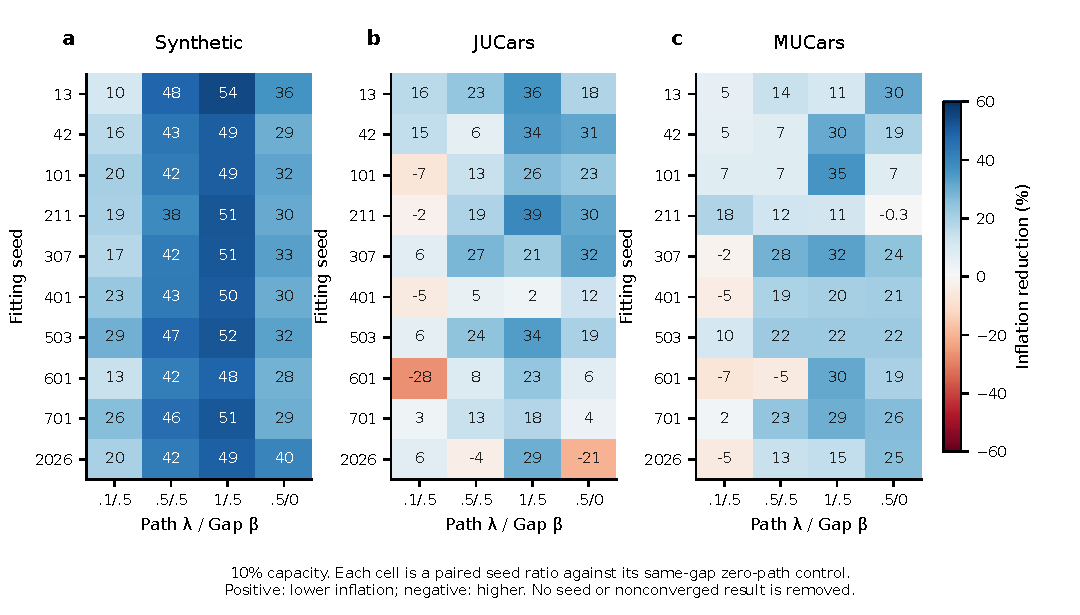
\includegraphics[width=\textwidth]{figures/ten-seed-v1/seed_consistency.pdf}
\caption{Ten-seed heterogeneity at 10\% capacity. Positive values mean lower inflation than same-gap zero-path controls. Negative effects and nonconverged responses are retained. Labels are rounded; exact values are in the public source CSV.}
\label{fig:rpl_seeds}
\end{figure}
\begin{figure}[tbp]
\centering
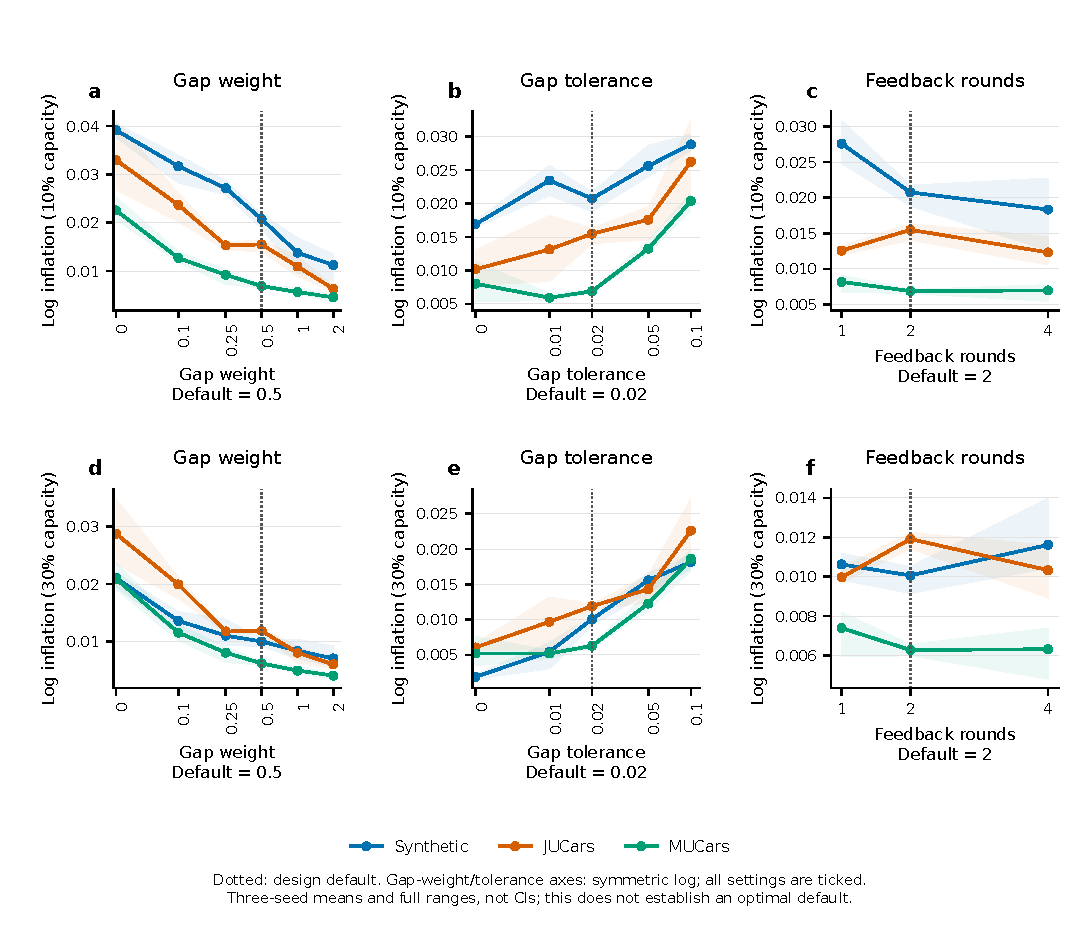
\includegraphics[width=\textwidth]{figures/ten-seed-v1/parameter_defaults.pdf}
\caption{Core-parameter scans in the original feedback implementation, with three fitting seeds. Dotted lines mark design defaults and all evaluated settings are ticked. Gap weight and tolerance use symmetric-log coordinates. Means and full ranges are descriptive, not confidence intervals. The defaults are engineering choices, not evaluation-selected optima.}
\label{fig:completion_parameters}
\end{figure}
\begin{figure}[tbp]
\centering
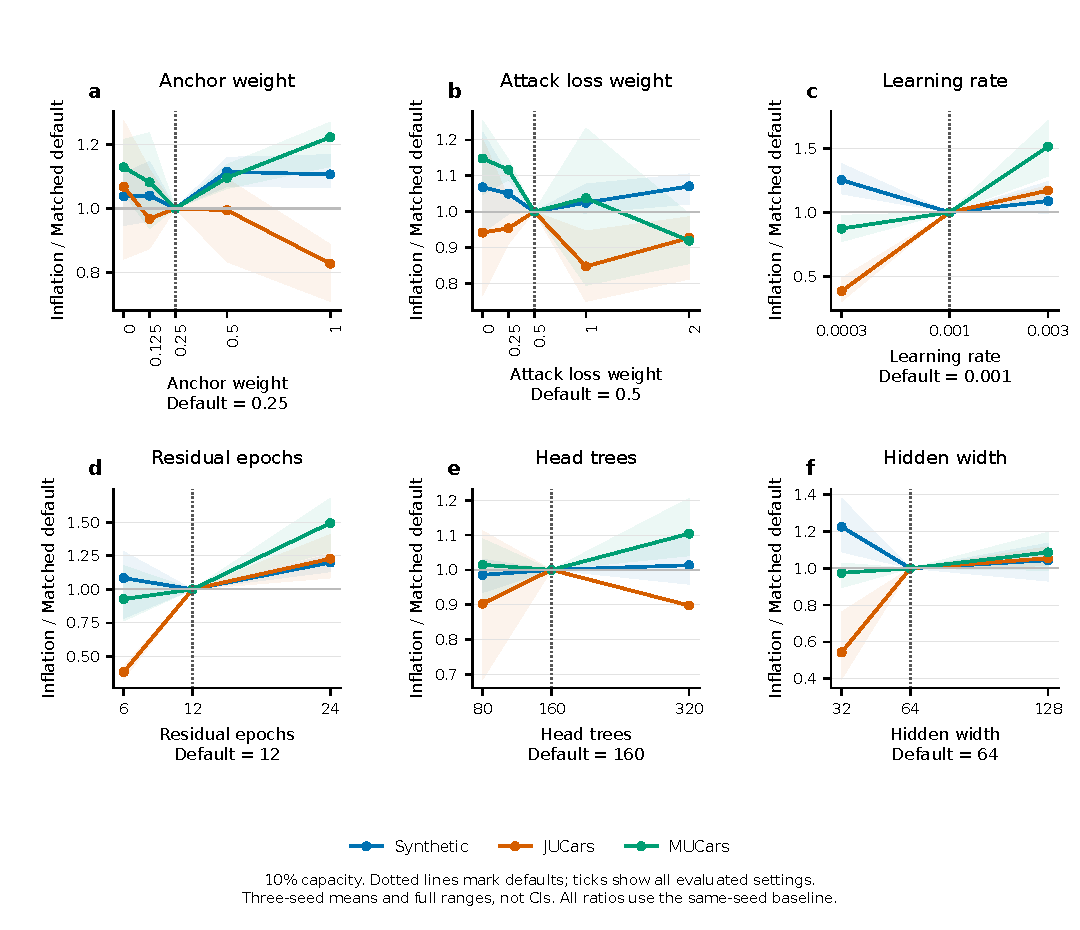
\includegraphics[width=\textwidth]{figures/ten-seed-v1/implementation_defaults.pdf}
\caption{Six implementation-parameter scans at 10\% capacity, retaining three fitting seeds. Every ratio uses the same-seed matched default. Dotted lines mark defaults; ticks show all evaluated values, and learning rate uses a logarithmic axis. Curves show means and full seed ranges, not confidence intervals.}
\label{fig:completion_stability}
\end{figure}

\end{document}
